%%%%%%%%%%%%%%%%%%%%%%%%%%%%%%%%%%%%%%%%%
% The Legrand Orange Book
% LaTeX Template
% Version 3.1 (February 18, 2022)
%
% This template originates from:
% https://www.LaTeXTemplates.com
%
% Authors:
% Vel (vel@latextemplates.com)
% Mathias Legrand (legrand.mathias@gmail.com)
%
% License:
% CC BY-NC-SA 4.0 (https://creativecommons.org/licenses/by-nc-sa/4.0/)
%
% Compiling this template:
% This template uses biber for its bibliography and makeindex for its index.
% When you first open the template, compile it from the command line with the 
% commands below to make sure your LaTeX distribution is configured correctly:
%
% 1) pdflatex main
% 2) makeindex main.idx -s indexstyle.ist
% 3) biber main
% 4) pdflatex main x 2
%
% After this, when you wish to update the bibliography/index use the appropriate
% command above and make sure to compile with pdflatex several times 
% afterwards to propagate your changes to the document.
%
%%%%%%%%%%%%%%%%%%%%%%%%%%%%%%%%%%%%%%%%%

%----------------------------------------------------------------------------------------
%	PACKAGES AND OTHER DOCUMENT CONFIGURATIONS
%----------------------------------------------------------------------------------------
\documentclass[
11pt, % Default font size, select one of 10pt, 11pt or 12pt
fleqn, % Left align equations
a4paper, % Paper size, use either 'a4paper' for A4 size or 'letterpaper' for US letter size
%oneside, % Uncomment for oneside mode, this doesn't start new chapters and parts on odd pages (adding an empty page if required), this mode is more suitable if the book is to be read on a screen instead of printed
]{LegrandOrangeBook}

% Book information for PDF metadata, remove/comment this block if not required 
\hypersetup{
	pdftitle={Title}, % Title field
	pdfauthor={Author}, % Author field
	pdfsubject={Subject}, % Subject field
	pdfkeywords={Keyword1, Keyword2, ...}, % Keywords
	pdfcreator={LaTeX}, % Content creator field
}

\addbibresource{sample.bib} % Bibliography file

\definecolor{ocre}{RGB}{243, 102, 25} % Define the color used for highlighting throughout the book

\chapterimage{Images/orange1.jpg} % Chapter heading image
\chapterspaceabove{6.5cm} % Default whitespace from the top of the page to the chapter title on chapter pages
\chapterspacebelow{6.75cm} % Default amount of vertical whitespace from the top margin to the start of the text on chapter pages

%----------------------------------------------------------------------------------------

\begin{document}
	
	%----------------------------------------------------------------------------------------
	%	TITLE PAGE
	%----------------------------------------------------------------------------------------
	
	\titlepage % Output the title page
	{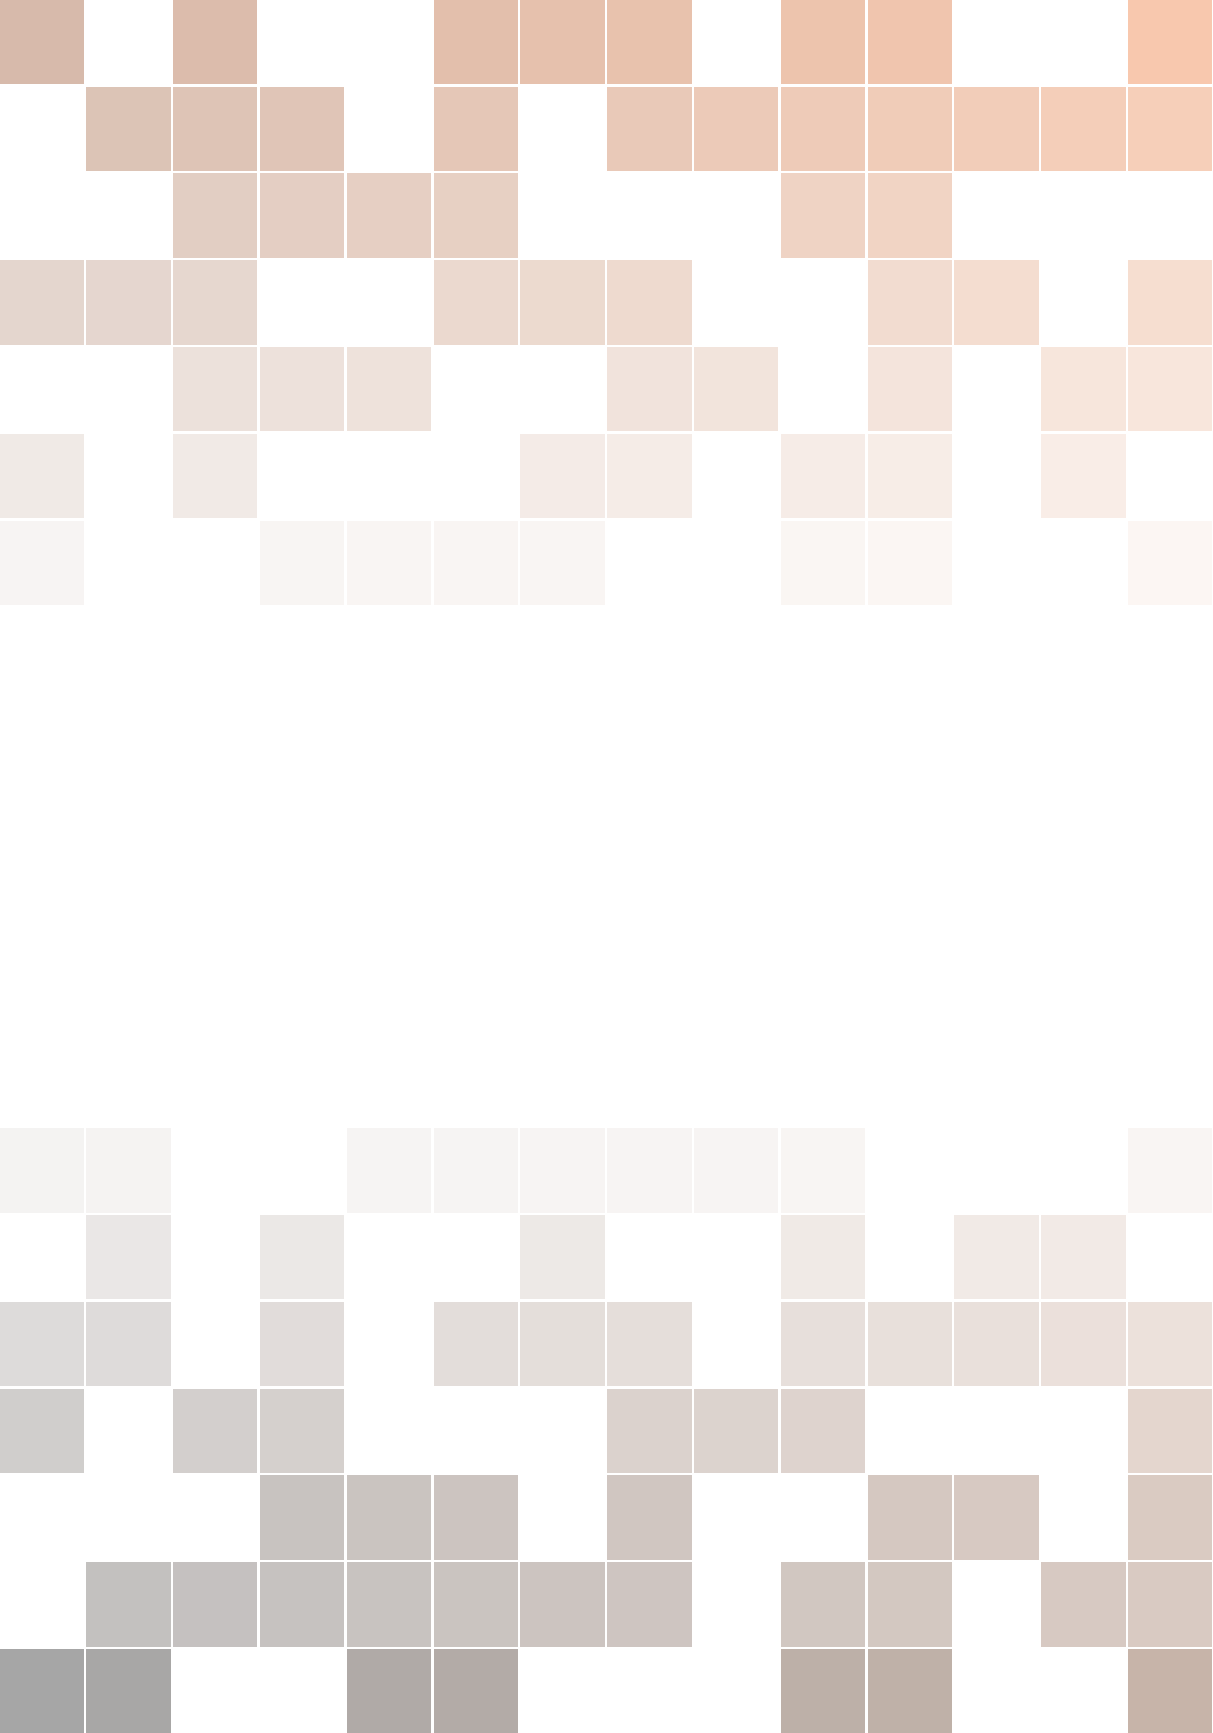
\includegraphics[width=\paperwidth]{Images/background.pdf}} % Code to output the background image, which should be the same dimensions as the paper to fill the page entirely; leave empty for no background image
	{ % Title(s) and author(s)
		\centering\sffamily % Font styling
		{\Huge\bfseries Micro and Nano Systems Track\par} % Book title
		\vspace{16pt} % Vertical whitespace
		{\LARGE A Micro Journey in a Nano World\par} % Subtitle
		\vspace{24pt} % Vertical whitespace
		{\Huge\bfseries Lorenzo Vergata\par} % Author name
		%\vspace{6pt} % Vertical whitespace
		%{\bfseries Whisper Large V3\par} % Author name
	}
	
	%----------------------------------------------------------------------------------------
	%	COPYRIGHT PAGE
	%----------------------------------------------------------------------------------------
	
	%\thispagestyle{empty} % Suppress headers and footers on this page
	
	%~\vfill % Push the text down to the bottom of the page
	
	%\noindent Copyright \copyright\ 2024 Lorenzo Vergata\\ % Copyright notice
	
	%\noindent \textsc{Published by John Doe}\\ % Publisher
	
	%\noindent \textsc{\href{https://www.latextemplates.com/template/legrand-orange-book}{book-website.com}}\\ % URL
	
	%\noindent Licensed under the Creative Commons Attribution-NonCommercial 4.0 License (the ``License''). You may not use this file except in compliance with the License. You may obtain a copy of the License at \url{https://creativecommons.org/licenses/by-nc-sa/4.0}. Unless required by applicable law or agreed to in writing, software distributed under the License is distributed on an \textsc{``as is'' basis, without warranties or conditions of any kind}, either express or implied. See the License for the specific language governing permissions and limitations under the License.\\ % License information, replace this with your own license (if any)
	
	%\noindent \textit{First printing, \today} % Printing/edition date
	
	%----------------------------------------------------------------------------------------
	%	TABLE OF CONTENTS
	%----------------------------------------------------------------------------------------
	
	\pagestyle{empty} % Disable headers and footers for the following pages
	
	\tableofcontents % Output the table of contents
	
	%\listoffigures % Output the list of figures, comment or remove this command if not required
	
	%\listoftables % Output the list of tables, comment or remove this command if not required
	
	\pagestyle{fancy} % Enable default headers and footers again
	
	%\cleardoublepage % Start the following content on a new page
	
	%----------------------------------------------------------------------------------------
	%	PART
	%----------------------------------------------------------------------------------------
	
	\part{Semiconductor Nanostructures}
	
	\chapter{Magnetostatics}
The course is trying to bridge the gap between a fundamental aspect of magnetism and the real application of magnetism in real life. And I was just making this example that's been between you as a student from my group who is really working to the redesign of the magnetic field sensors. But for doing this he needs all, I'll say, all the ingredients that I tried to explain during this course. That's the reason why he's attending the course because it's not coming from physics engineering. So this course was missing in his career. A friend of mine, who's not just a friend, he was the past president of the European Magnetic Association, the name is Burka Hillebrand, who is the father of Magnolian Westerners, who is used to say that Ricardo, you have a double soul. You are a physicist but also an engineer. Obviously it's true, my degree is in electronic engineering, but in the end my PhD is in physics and I'm giving a lecture in physics. But okay, what I try in my life is really to establish sort of a bridge between academia and companies and so on, because this is our real life at the end of the day. Mathematics is very beautiful, but what is the day-by-day implication of that? Now I will try during this course to make some example which really can be used to bridge the gap to show how quantum mechanics begins real application also in the field of back end of production.\\
Basic magnetostatics, which is now the topic of today's lecture. Understanding what happens in statics. Magnetostatics means state-stage system. We are not talking about in waves, permanent regression dynamics, static configuration of a magnetic bond. which means not just iron and an infinite crystal, but a piece of iron. It is shaped as a sphere, the film, the bar, the shape makes the difference. And magnetostatics deals with the static configuration of the magnetization, not the field created by the magnetization. In some sense, this is the physics of three magnets. Okay, when you have a three magnets, you can play with magnets. And you know, if you know this game, which is your mind. You're playing with German. Yeah, that's a good starting point for this. Get to play. So you understand the magnetic force magnetism. And what's your name? I sound good. That's the names of today. It's been so let's start with when you play with the German. I give Pearson is the right-hand pole, he is the left-hand pole, North, North, and South Pole. So we have to understand the physics of the geometry. Okay. First of all, let's review which are the main characters of this course and the basic equation that you have.
\fig{2}{lecture_1 basic magnetostatics.pdf}
So you have different characters and things. B, H, and L. Okay. Well, the three guys are feeling this one. B is the induction field. H is the magnetic field. M is the magnetic solution. Let me just review the meaning of this. Which is the difference? Sorry. I apologize. I apologize. M is the magnetization. What's the definition? It's the magnetic moment that you are holding. Magnetic moment that you are holding. So what does it mean? How do you measure a magnetic moment? Magnetic moment, you should always refer to the idea of the circuit, so the magnetic moment is measured in water. It's the intensity of the current multiplied by the area. And when we go to the magnetization, we need to realize that magnetization is measured in water. Current by surface divided by volume, to the current divided by a light. That's why in terms of units, it is measured in amps per meter. That's the unit of the magnetization of the International System of the Universe, in which we will live and be. I made this choice in the very beginning, not purely for the different systems that I'm using in physics. I'm using now the International System of the Universe. amps per meter. And then you have the induction field B and H. I ask you, what is the difference between B and H? I do not completely agree. the example for HF. Okay, the relation is this one. B is equal to 0H plus F. Okay, that's the definition. But physically, you have to say what is the difference between B and H. But for that, B is the vector appearing in the Lorentz field. So an electric charge is moving in a magnetic field with the Lorentz force, 2B cross B. and is B the field which determines now the force acting on the magnetic field? It is B. H is something slightly different because H is connected to what? The current. The connection is quite straightforward. You know that the curl of H is equal to J Not only this, but what should I have here? Maxwell equation, one hundred most beautiful things of every size, plus, plus root. Something is missing. Yeah. You can write in the free space or otherwise you can write in the derivative of D, with respect to the time. But for today, if you write in magnetostatics, you can also forget about this one. Magnetostatics means the states of the oscillation of the coordinates of the light and the field is not changing. But you immediately see that H is directly connected to the source of the magnetic field, which is usually connected to the current flowing in a wire. But this is not the unique vision of the story, especially magnetostatics, also because when the free space but their current amount, no. Obviously, the field is going to be better. And what is now the problem or the opportunity? The opportunity is here, B, as you see, the museum, EH plus M, okay? So, and the H can be reduced by the magnetization itself. So, what is the Fritz magnet? The Fritz magnet is made of an odd magnet, typically a cobalt, a boron, or a chloride, which displays a nice, realistic look. So, at zero, external field, you have a net Riemann magnetization. And so, this is the source of the H, okay, especially magnetostatics. In magnetostatics, when you say What does it mean? There are no currents of one in the center. That's the framework in which we are more. So the the derivative we expect to time are equal to zero and no current. So the sources of the magnetic field are not connected to cards, but connected to the presence of the body which is magnetized in remnants due to the fact that it's a full magnet due to exchange interaction with a remnant magnetization at zero external field. And that's the reason why when you move from there to this relation here, you usually find that B is equal to mu zero, HM plus M. And this subscript M is here just to tell you that this is the H field not produced by the current here. The J zero here, okay, is produced by the magnetization itself, okay? So no current means that the H is not produced by J. So this means also that the curl of H equal to zero. Okay? This is zero. And that's the reason why in magnetic structure, at values with the general framework of electromagnetic you can define what is gamma retention. The reason is quite heavy, it is immediately evident. If you see that you have a vector h whose curl is equal to zero, but this means that you can write h as the gradient of something else, a kind of field, exactly as in order as in order to start. So you can say that, okay, so if this is the story, I can write immediately H is equal to minus the gradient of a scalar potential U. Usually you cannot do that. So the kernel of H is equal to U, not because we are trying to use the vector equation. But this is not the case. Here you can use a standard equation. And there is another story which is also relevant here. In terms of units. I didn't feel completely stable here. M is the magnetization which must be expressed in m per meter. But according to this equation here, here, m and h, they have the same units, okay? This is quite evident. So h, again, in amps per meter, so if you want this magnetic field, and this is the induction field. and the magnetic field must be measured in m per meter and as you have this pointed here this constant which is near zero which is the back of the mobility 4, 5, 8, 10, 11, 17 units in the initial system it does all that it also has it's not dimensionless this one So then the unit for B is Tesla, okay? In the international system of units. B is measured in Tesla, M in the international system of units. Okay, so these are the three characters of magnetostatics. The basic equations are these two equations here, and from these you immediately realize that you can use the scalar potential, which is much easier for multiplication. Scalar potential. And now, what's the impact of this? Immediately you realize that you can apply the same mathematics over the rhythm of statics. So we have the scalar potential, h is minus the gradient of u, which is like the case of e, given to e, but minus the gradient of p. And so, okay, and so. And so what happens? You can say okay, but if you have this equation here, you immediately find that you can write down a Poisson or Laplace equation for the magnetic star hypotension. And how it goes out? So it's very simple. So do not forget that B is always true that the divergence of B is equal to zero. Because there are no magnetic monopoles. The divergence of B is always C. So essentially, you have it, okay? The divergence of B is equal to zero, but B is mu zero by H plus M. This means that the divergence of H is equal to minus the divergence of M. Okay? And then instead of H, you can replace minus the gradient of U, and this means minus the number of squares of U, which is equal to minus the divergence of M, and so your your language with this equation. The Poisson equation, okay? The Poisson equation is the number of squares of Q which is equal to the divergence of M. It's very similar to something that you know. Number of squares of B is equal to minus O divided by epsilon Z. Okay, it's again a Poisson equation. And so from the analogy that I started to tell you about, this seems to be related to sort of charge. And indeed we will see that it's exactly connected to the concept of magnetic charges. But okay, let's continue this discussion. So we are here, we have this equation here, It's a sort of Poisson equation. Inside the magnetic body, you have a diagonal. You have an M, okay? Don't forget that in general you have a magnetic body with a volume, surface, and the norm under the surface, N, according to this. And inside the body, you have a non-moon diagonalization, so you can have a 30-D-L. It can be zero or not, depending on the divergence of M. But you can have it. But outside the magnetic body, there is no M, M is zero, the divergence of U is zero, then you have not a Poisson equation, but a Laplace equation. now the square of u outside must be equal to zero. And now you have this Laplace equation plus some equation. That's a typical problem that we have seen in electrostatics, and so one can say it's the answer. Of course, we have some boundary conditions, because we have an equation inside, an equation outside, now without the boundary conditions. We will see afterwards that the boundary conditions for U at the surface are these two conditions. The continuity of the U is very similar to the continuity of the electric field. The electric field can admit this continuity, not the tension, otherwise there is a divergence. And there is another condition, which is this one, stating that if you calculate now the derivative, the direction of the derivative, the derivative of u with respect to the direction to the norm of the derivative inside, you subtract the same direction of the derivative outside, immediately inside, immediately outside, this is equal to m dot. We will see that this is exactly the same condition that you are used to, stating that the normal component of B must be conserved when you cross a little bit between the two points. But okay, you have this regulation, and you have this binary condition, and provided that you find a solution which is regular at infinity, which corresponds to this condition here, condition, a fantastic condition, a fantastic situation, so that if by inspection you find a solution, that the solution is not a second solution. This genus theory is an extremely powerful tool for solving magnetic static. And this is a very powerful method for solving the problem that we will see.
\fig{3}{lecture_1 basic magnetostatics.pdf}
Now, as I was telling you, this is a negative sign. That could be also an exact sign. That's exactly this one. So, demonstrate that the boundary condition that you are used to from general courses of the electromagnetic state in that when you cross an interface, the parallel component of H and the perpendicular component of B, not B, show that these are equivalent to the following conditions, exactly the conditions I told you about. So let's solve this exercise, just to work it out. So one could start with the condition for the conservation of perpendicular components of B. So what happens? Let's imagine that you have neutral states between two magnetic materials, different magnitudes. This is inside, so let's imagine that, okay, this is your body, okay, so you are here, and here it's outside, okay. So the typical story that you know is that inside and outside the perpendicular component of B must be equal. So B in perpendicular must be equal to B out, okay? This is B. But now what about B? B is mu zero by m plus h. Inside you have m, outside you don't have m. So this is your body, outside you have a vacuum, but it's no magnetic material. So inside you have to write down mu zero m plus h m. Okay, inside. So, outside you have what? Mu zero, h m, no longer there. So mu zero, you don't need it. And now you have what? Okay, m. But you have to take what? The perpendicular component. So this gives y. So you take the projection on the normal, the unit vector which is normal to the surface, which is n. So let's assume that here you have this n. So you take m dot m plus volt. Okay, let me say that this hm can be written like minus, what is it? H is minus the gradient of u inside. So you have minus the gradient of u in dot m, u in dot n, which is equal to h outside, same story, minus the gradient of u out dot n. But when you take now the scalar product between the gradient and the normal, what are you find? r is the direction of derivative along the direction of the norm. You project the gradient in the direction to find the partial derivative along that direction, to the So, in the end, you have m dot n. So what is this? Minus partial derivative of u in with respect to n, equal to minus partial derivative of u out with respect to n. And this is exactly the condition which is reported there. So in the end you find out that the discontinuity and the partial derivative from inside and outside is equal to m dot n. Okay? Good. First condition, which is demonstrated, so the equivalence is demonstrated. you have a cycle one just that concerning the fact that the parallel component h in parallel might be concerned but be equal to h out of that and here i say what you say it is automatically satisfied i told you that h is equal to minus the gradient of U but okay this means that the curl of H is 0 okay no way curl of H is equal to 0 if the curl of something is equal to 0 it's very easy to demonstrate that you take a path like this and you integrate the curl this means the circulation over this line must be zero, and this automatically brings you to the conclusion that the true pilot component must be equal. Automatically . And then, what's the origin for the continuity of the U inside and outside? It's not connected to a very simple show. As H is equal to minus the gradient of U, It's evident that if you have a discontinuity in the U, you will have a divergence in H. And you want to avoid this divergence, which is unphysical. It's exactly like an electrostatic. In electrostatics, you can have a discontinuity in the electric field, but not discontinuity in the potential. So if you are discontinuating the electric potential, there is a divergence of the electric field at that boundary. here is exactly the same thing. So when you write down these conditions, you ensure that H is according to which is well defined without divergence, and you are ensuring that the parallel component of H is conserved and what's the curtain in your component is conserved. Okay, so this is an exercise that I'm used to to solve. Are you okay? What's the name? You also fear that you won't qualify. Sorry, just trying to recognize the face. So, it's an exercise just to make some practice with Maxwell equations, which could be also nice for restarting a little bit at the beginning of this course. OK, but now what's the point? We found that we have an equation which is nice, which is an equation in which you are essentially look at this part here.
\fig{4}{lecture_1 basic magnetostatics.pdf}
It's a Poisson equation. This slide is meant to establish a full analogy between magnetostatics and electrostatics. Look, for the magnetic material, we have that B is equal to 0H plus M. For a dielectric, we have that D is equal to epsilon zero by E plus P. What is P? is the polarization effect is measured in two more room meters squared. And so you see that there are three characters with some correspondence. So B, the meaning of D, the electric field H, and instead of M, you have B. And those are physically you understand that the meaning is very similar the polarization that you can have in the material has the same function the functionality of the magnetic solution and as a matter of fact the equation described in ferroelectrics and true magnets are very similar the long dowel potential for both systems is exactly the same so the same properties can be you have a coercive field, an inferred magnetism, an electric field, you have saturation, remnants, you have a coercive field and also a loop, an integrated loop, anyway. Now, H is equal to minus, gradient of U, but E, the derivative is minus the gradient of H. One to one. There is a difference. The divergence of B is zero. That's a big difference. the divergence of E, the Gauss theorem, is equal to the density of charge divided by the density of E. But in terms now of the equation that you find, here you have the number square of U, which is equal to the divergence of M, and in that case, you have the number square of B is equal to minus 4 divided by absolute E. So, let's use now the thermo-centrifugal climate. The same equation has the same solution. How can you apply this central theory? Because, okay, what are you used to apply in eletrosclerosis to solve the problem? You say, okay, I have this equation. Now, forget about the left problem. Now, the density of charge that we put there is the sum of two contributions. We can have three charges, those appearing at the surface of the components, and polarization charges, those appearing in dielectrics, either at the surface or even in the volume, depending now on the condition of polarization of the volume. But what is the solution for the problem of the electrostatic? We can write down the expression for the potential, starting from the superposition principle and the solution for one charge. So that you can say that as the source for the electric field are water, the potential, the free charges on the conductor and the polarization charges, we can write down this equation saying that okay the road to be placed here is the sum of three row three density of charge minus the divergence of the example is the way you write down the density of polarization okay so let's assume that row three is see what you see. I'm not coming back to it. So I just left with a dielectric material which is polar. It's exactly what you have on this side for the main of the star. You don't have electric current here. The equivalence story is we don't have electric charges to the mass. So, the Poisson equation becomes the number squared of V is equal to minus by minus the state of space plus the divergence of space divided by epsilon. This is the equation, and the solution is something that you know very well. The solution is this one. V is equal to one divided by four pi f multiplied by one, the sum of two into one. The first one is the contribution to the electrostatic potential coming from the volume of the charge. C minus the divergence of P in the R-th parameter, divided by R minus R-th, contribution from the volume charges of polarization, plus the contribution from the surface charges of polarization, P dot n. Okay, this is the really the surface density of collision charges divided by r minus r prime integrated over x. This is the solution of the equation. But now you can say, okay, the density, the volume density of collision charges is minus the derivatives of p and the surface density of collision charges is p. Now you go back and say, okay, but here I have this equation and the other equation. So now you can say, okay, same equation, same solution. Strong parallelism, you say, okay, let me write down instead of v, u. Here you have 1 divided by 4 pi epsilon zero. Okay, here you have epsilon zero, here you don't have something at the denominator. So just 1 divided by 4 pi, multiplied by the sum of two integrals. The first integral would be a volume integral, same here. divergence of P, but P, in this case, is m, so minus the divergence of m, divided by r minus r prime, integrated over the surface. Then you move to the integral over the surface, that was here P dot m, what do you find here? m dot m, divided by r minus r prime, integrated over the surface. And that's the solution for U. You see the strong analogy between the two things, same equation, same solution. So you have found now the connection between the magnetization and the U. And the problem is solved once forever, because now if you know the distribution of M, you You can calculate the U and if you can calculate the U, H is equal to minus the gradient of U. End of story. You see my point? The problem is solved. And now there's another column. Do you have a question? Yeah. I'm not sure. Yeah. It's another idea. Right. Is the analogy so that when we are talking of charges in the dielectric field, the corresponding is the charges and the corresponding is current. Exactly. So, by analogy, volume and energy charges are current in this case. Are you referring to this slide? Yeah. So you're asking me something before I explain that. Just go. What is that? I have something. I have something. I have a signal. I have something. Okay, one neuron remains. It's a big issue. Sorry. Okay. Let me first make a comment and then probably the solution, the question, the answer to to your question should be quite clear. Let's now make a comparison between this solution for U and that solution for V. You immediately try to associate this minus divergence of M with the minus divergence of P. But as minus divergence of P is the density of polarization charges, You introduce this concept, which is a pure mathematical concept of volume magnetic charges. As you see, minus the radius of P is physically a volume density of the partition charges. Okay, so this term, BA, is like a volume density of something that I call by analogy magnetic charges. Do magnetic charges exist? No. It's just a pure mathematical concept that you are using in order to explore the analogy. Okay? They do not exist. So the divergence of B is equal to zero. Okay? only the Naomi dipole exists so far, okay? Who will demonstrate something else with the normal price, millions of dollars, for the time being, is pretty much equal to zero. So this means that it is just a mathematical term that is useful and can be helpful when you try to solve a problem, but it's a mathematical term and by analogy. What about m dot n? p dot n is a surface polarization charge density. So you say that m dot n is like a surface magnetic charge density. Okay? Why it's so relevant to your theory? not everybody loves this kind of approach. People say, okay, now you have to use the vector potential in a way, why are you running with the scalar potential? But in practice, you will see in a while that establishing a sort of parallelism, like the static problem, ending with a static one, is very powerful because it because it provides you with an immediate vision of what is going on in the magnetic field, starting from the concept of the electrostatic process. You know very well, you are not used to work with magnets, you are more used to work with electric charges, potential and so on, so you can now use what you know from the electrostatic and apply it to you. That's more or less the A very simple example would be this one, and then we will take a break, otherwise the lecture will become too long. So you know what's the origin of magnetism, of the name magnetism? You know the origin. You know magnetite. Magnetite there, okay, what is magnetite? It's a rock, okay. So magnetites come from magnetite, okay, but which is not the end of the story. to magnetize In iron free Is a rock but who gave the name magnetized to this rock With bricks they did they gave the name to her to everything They just they discovered everything and also the final that we were just making something final everything was done by greeks So yeah, the Greeks, which Greeks living in which city? Is he famous? Was he a philosopher? Okay, but he's connected to Magnetism. It's Magnesia, the city of Magnesia. Magnetism comes from the city of Magnesia, Magnetism comes from the city of Magnesia, in Italy, the station of Magnesia. And that magnetism came. They discovered the property of this rock around the 7th century B.C. And they were typically playing with this rock shaped in the form of a bar. Like in the German. For a reason that I will explain in a while, when you have a bar or a through-magnetic body, it displays a natural tendency to develop the remnant magnetization along its axis, Which means that you can imagine that M is uniform and is directed along the axis. But now let's imagine that you have a cylinder which is uniformly magnetic. Quite low. Do you have some magnetic charges inside or at the surface? Let's imagine that it is uniform. there are no volume magnetic charges, so the divergence of M is 0. No magnetic charges inside. Are there some surface magnetic charges? So you have to calculate M dot N. And now you have two possibilities. This is N here, but M dot N is 0. zero, you don't have magnetic charges on the surface, on the lateral surface of the cylinder. Nothing. Zero. But what happens here? Here you have N1 and here you have N2. And you discover that M dot N1 is positive and on the other side you have sigma 2 which is m dot n2 which is negative. So you can now say that mathematically you can think about some positive magnetic charges here, some negative can be charged there. And now let's imagine that you have a problem like this in a leg of a car. Which kind of field do you expect to see? You know the solution. The field lines are expected to be like this. Which is exactly the solution for the magnetic field produced by a valve end. That's the reason why he played with the German. Because if you have a cylinder which is uniformly magnetized along the direction of heat, Hartz's, you just have some magnetic charges concentrated at the two extreme portions, at these two phases. So these are the the north and south poles interacting differently, okay? Positive and negative charges. Two positive poles, they repel each other. Two poles with opposite sides. But, I think it's exactly this. And this is just a pretty simple example explaining why disposable magnetic charges can be very, very helpful. We will review his many, many facts, but from now on, we will leave it. quantitative and elegant way.
\fig{5}{lecture_1 basic magnetostatics.pdf}
So essentially we have the problem of an infinite cylinder with an axis along z in this x, y, z reference frame. And let's assume that the infinite is physically, unphysical, but it's a mathematical simple problem describing a long cylinder. It is the same that I just tried to solve here, in which we are putting the charges far and far away. Now M is uniform in size. It means you take the magnetic material, you shape it into a cylinder, you magnetize it in the Z-direction and okay, the problem is there. Which is now the magnetic field. The B is H, produced by this distribution of magneticization. So we know that the equation is always the same with the Poisson equation, but in this case, as M is uniform inside, We can't argue that there are no quantum magnetic charges, that the Poisson equation becomes a class equation. The number of squares of u is equal to zero. And the general equation of this is what? The number of squares of u is equal to the divergence of m. But as m is moving from the inside, the radius of m is 0, and we are left with a log-Nagel situation. Clearly, in this case, it is useful to work in cylindrical coordinates. The double-square assumes this form. When you are using rho, which is the radial coordinate, phi, which is dv, the azimuthal hangar here in the x-1 plane, and z, of course, which is the coordinate of the axis of the plane. So this is the representation of the Laplace equation, and what about the boundary conditions? Boundary conditions here are connected to the possible presence of modes of magnetic charges. But in this case, you don't have magnetic charges. reason is quite simple, because m dot n is equal to zero, m dot n, they are perpendicular. So there are no magnetic charges on the lateral line of the solution, okay? No charges there, and in this case, there are no magnetic charges at the top and at the bottom, because at the top and the bottom, they do not exist. They are an infinite cylinder, or they are put at infinite So boundary condition becomes this one. So there is a continuity in the partial derivative with respect to the n, which is the body of the constant. And you know that you must have a complete condition. How do you solve this equation? Don't forget that if the solution exists, it's unique. What is the trivial solution of that equation? Respecting the boundary. U equals the constant. Okay? Because if U is equal to the constant, perfect in the sense that, okay, the equation here is partial derivative equation, equation, the automatic density is zero. And, of course, the two partial derivatives equal to zero, and there will be a continuity of the U from inside to outside. So, immediately you find that this simple solution that you see by height, by inspection, is U equal to zero. Okay? And now what is the implication of u equals to zero? What are you looking for? You're looking for h. h is minus the gradient of u, which is equal to zero. So what's the implication? h is equal to zero everywhere. Okay? Everywhere. Does it make any sense to you? You have a material which is uniform and magnetized and if it is linear and H is equal to zero Is it possible that it makes sense? Or some Is Can you find any connection between this problem and that problem? This one. This problem transforms into that problem if you do what? If you put these two faces at minus infinity and plus infinity. But what's the impact? We have magnetic charges at infinite distances that do not create a magnetic field where we are. You see? But in case of the 11th time, if you have some elliptic charge that place at plus infinity and noise infinity, it will not produce a 5, it will be a ui. You see the point? So it makes sense. Here, it makes sense. So you have that H is 0 everywhere. What about B? Is it 0, B? No. So, B. So, H is equal to zero, but B is equal to mu zero H plus M. So, you have B is equal to mu zero M. So inside the cylinder, you have m and you have b, and they are parallel. b is equal to mu0, but we don't have h. So h is equal to 0, and h must respect the statement as the surface, there must be a continuity in the parallel to the point of h. If h is 0 inside, it's also 0 outside. But let's go back to the other. This is for an infinite cylinder. And in that case, in the previous one, this was H out. What about H inside? In the case of a finite cylinder, H inside. could be now the orientation, the direction of age inside? What's your name? Sorry. Eduardo. Eduardo. What do you mean? From right to left or from left to right? But so it all this proposed in like this age in Do you agree What's your name Why do you say the opposite you have to H parallel inside and outside, they must be equal. So it's impossible to add this. You see my point? That's impossible. Because this will violate the conservation of the tangent of the parallel component of H. So, H inside would be like this. And this is totally coherent with the analogy with electrostatics. Because in electrostatics, the electricity goes from positive charges to negative charges. And in magnetostatics, it's exactly the same. The magnetic field H goes from positive charges to negative charges, both inside and outside. So this is the unique possibility that you have. Pay attention to one fact. H inside here opposes the magnetization. That's the reason why it's called demagnetizing field. the fact that you create a surface, it creates some, so you're creating some magnetic charges at surface, and they generate a field which opposes the magnetization. It's a demagnetizing field, which tends to demagnetize your body. Okay? Okay. So coming back here, that's the reason why you say H in is also called H demagnetizing or HM or H in. Demagnetizing field, magnetostatic field produced by the magnetization or H inside. Just different names. But this is a very fundamental concept. So there is a demagnetizing field, which opposes the magnetization, due to the fact that you have some surfaces. You have a finite volume to be applied by the magnetization. In case of the infinite cylinder, there are no magnetic charges, so, the charges are plus infinity, minus infinity, they are not able to create a demagnetizing field here that's equal to Z. So then B is equal to mu zero by N. So in this sense, the maximum B that you can have is that for an infinite cylinder. Because you are during the demagnetizing field. Okay? And then, okay, there is a strange story here that we have to review in a while. Let's see, so EM, what is EM? EM stands for magnetostatic energy. Something that can be seen is that the magnetostatic energy in this case is equal to zero. I will try to review this concept afterwards, after explaining in more detail what is magnetostatic energy.
\fig{6}{lecture_1 basic magnetostatics.pdf}
Let's solve another problem. Just very, sorry. Yeah, this one is very similar to the previous one Jogging is exactly the same In your infinite cylinder that you're ready to are but now it's my it is magnetized along X direction to the right of it Big magnet and the other song and the top three it can be my reward the magnetizing on the x-axis. But now what's the field produced? Are these perfect or not? The question is completely, but now you expect to see some magnetic charges on the moon. Now same machinery and you say okay So this is the first case second case here Nothing changes here. Okay again M is uniform inside which means that the equation is always the same Yeah, then Navla squared of U is equal to 0 now the boundary condition So the equation is always the same but the boundary condition are different The boundary condition is the boundary condition are expressed like this So Let's me do something This X is Y and then this point towards you. Okay, so this is a cross-section In your circle radius are So it's not very good The magnetization is Pointing please This is m. Okay. And now, let's write down the boundary condition. Boundary condition is saying that the derivative of u in psi with respect to r does it... Let me say that, for instance, I'm taking this angle, which is the angle phi, the n as a normal, like this. Okay? And so when I take the partial derivative with respect to n, I'm taking the partial derivative with respect to the value of the insulated asymmetry. So it is the partial derivative with respect to n inside, minus the partial derivative outside, with respect to r, must be equal to m dot n, okay? What is m dot n? It's m by the cosine of the angle of 5. Okay? m by the cosine of the angle of 5. Now, we are left with this boundary condition, and And so one could say u equal to zero cannot be a solution. It doesn't respect boundary condition. You will have zero equal to something that is not zero, not everywhere, so it cannot be a solution. And by inspection, we can easily find that a solution could be this one. I understand that you have the light here is creating some problems, so let me provide solution, so the u, the function of r, can be written as ms divided by 2 with, okay, now, the nightmare for you, being kind of in here anyway, there's no problem. So ms divided by 2 by the cosine of the angle phi, okay? And now, if you are inside, inside the cylinder, you multiply by half, by rho, or by half, same story. Or, you have ms divided by 2, again cosine of phi by r squared divided by r. Okay, in case r is larger than capital R. And you find it's a solution, it's quite easy. If you replace this one inside the equation, you find that it is . equation, which has the previous substitution and so on. But now, if this is a solution, what is going on? First of all, you should recognize something which is very similar to an electrostatic problem. So if you try to plot this, you will discover that the u is a function of r. It's like this, okay? Something that you're used to with the equation. Okay, and after that, there is a continuity, so everything is respected in terms of the goodness of the solution. It's a good solution, this one. And so it's a unique solution, but what happens in practice, which is now the field that you have inside? Okay, now this is the u, so let's calculate now the h inside, okay? okay, and iterate it in the H inside. What you can say is that H inside should be what? Minus the gradient of the U inside, okay? Which means minus the gradient of this quantity here. But when you have this cosine of phi by R is exactly what? is the x coordinate of the point. It's x. You see, the projection of R on the x-axis. So, it's a gradient of ms divided by 2 multiplied by x. And this means that the field H in will be equal to what? Just minus ms divided by 2, multiplied by the unit vector of the x-axis. So there are no other components. So it turns out that m is pointing along the positive direction of x, h inside, which is also hd, the demagnetizing field, is pointing upwards And what's the reason of this? You want to apply now the analogy with the electrostatic? That's quite easy. What about the surface magnitude charges? m dot n here is positive And m dot n here Assume that your n is pointing this is negative. So the demagnetizing field, the magnetostatic field is pointing from positive charges to negative charges, both inside and outside. Inside, that's a very interesting property, I want you to notice this one. Inside, we have M which is neutral, also H is neutral. H is minus ms divided by 2. Okay? It's uniform. Outside, the story is different. Because here we'll have some field line, but we'll try to do something like this. This is outside. Of course, you have a symmetric situation here. But inside, the field is uniform, and its value is minus ms divided by 2. the minus 10 for the project, you have a different design in the world. You don't have that divided mind. That's a very pedagogic example. You have the same geometry in the city. You change the direction of the magnetization, and the physics is completely different. It's always high-voltage, it's always a very high-voltage, but the film produced is completely different. Start seeing the impact of the shape and the fact that you don't have an infinite crystal, you have a body with a shape. And of course, okay, there are no other components here, and we want to calculate this magnetic attraction, but I will do that afterwards.
\fig{7}{lecture_1 basic magnetostatics.pdf}
Third example, a sphere. A sphere. We are seeing very simple shapes, but you will see that the sphere, for instance, is not just an exercise. So far, there are just two examples of devices, commercial devices, exploiting magnetic spin waves, or dynamical processes in the magnetization. One of them is that of the reference oscillators used in the Gigahertz range by a company working with telecommunication and radio frequency application and so on. And the basic component of this is a sphere of Yttrium Iron Gun. The reason why it's a sphere is something that I will explain later on. Let's start from this regard, that is, the code here, which comes from the solution of the equation, the Poisson equation that we worked before on the black sphere. Of course, in a sphere, there is the full symmetry, which means you can rotate it as you want. Let's take now a reference frame like this one. Let's assume that M is pointing along the center. here uniform with micro-diameter. The story is always the same. If m is uniform, the divergence of m will be equal to zero, which means that you're left with the Laplace equation. The nabla square of u must be equal to zero. Everywhere, inside and outside. Outside because m is zero, inside because m is zero. The divergence of the uniform field is zero. Now you write down the equation, the Laplace equation in spherical coordinates, which has this form over there, and you put boundary condition. Now what about boundary condition? Now just to, quite simple, just to give you, to clarify the meaning of the angle here. X Y and Z now let's take this direction of the magnetization to the angle theta This is the angle phi. This is the polar angle theta, and this is the angle phi defining the direction of the magnetization. Sorry, the direction of n in this case, not of the magnetization, of the norm. m is always pointing along z. But n is pointing along whatever the direction. So when you write down the boundary conditions, the partial derivative of u in respect to n minus the partial derivative of u out respect to n must be equal to m dot n. And so you immediately realize that this is the polar angle theta which comes into play. So you have this is equal to m by cosine of the angle theta. This is the example of this equation. And then again by inspection, you find out that the U inside would be equal to ms divided by 3 by the cosine by r by the cosine of the angle theta. It is inside, okay? But r by the cosine of the angle theta, it gives you exactly the z coordinate of the point that you are considering. And so when you calculate now h inside, which is equal to minus the gradient of u inside, it turns out that you are selecting just the z component, and it will be equal to minus ms divided by 3 multiplied by uz. Okay? So again you find the concept of the demagnetizing field. Because M is pointing up here, along Z, and the demagnetizing field will be like this. Minus M s divided by three. Okay? And that's another example of application in this machinery of the megawatt static field, the epi charges and so on. Again, you can say that you have some positive charges there, not negative charges on the other side, and of course the density of surface magnetic charges will change at a different polar angle. It would be exactly equal to zero in the equatorial plane, and it will become positive in the north hemisphere, and it will become negative on the other side.
\fig{8}{lecture_1 basic magnetostatics.pdf}
Now, let's have a talk of generalization of what we have seen, and I have five minutes. Let me just introduce the story, which is that of the ellipsoid uniformly magnetized. The basic observation of what we have seen so far is that all the examples that we have For all the examples, we put M uniform, and we found that the demagnetizing field was uniform. In case of the infinite-cylinder magnetized along Z, H was 0. It was a uniform field. In case of the cylinder magnetized in the radial direction, it was minus MS divided by 2. In case of the sphere, it was minus MS divided by 2. So one could ask himself. So this means that for every body, every shape, if I magnetize it uniformly, H, when I magnetize it uniformly, the answer is no. F is no. There is a theorem stating that if and only if the surface of the magnetic body is of a second degree, what does it mean, a second degree? the linear is described by the equation of second degree, the sphere is described by the equation x square plus, y square plus x square equal to r square. So only if the equation described in the survey is of a second degree, in case of m uniform, you find that the female determinant is equal to r. But only if this happens, we say the a is of the sphere, and in general, it's a case of another sort. For the equation in this one, where a, b, and c are the all-axis along the different x, y, and z axis. Now, in this case, you can write in general that h is uniform and can be connected to m by this very simple equation in which you have this N, which is the tensor, so that H inside, or Ht, you might as well do this, is equal to minus N multiplied by M. But M is a minus. M is of course is a tensor, so it doesn't mean that both this, so it depends now how you put M, you find the direction of H. There is a theorem stating that if you properly choose the reference frame, the trace of n is equal to 1. And let's see now what happens in the three cases that we've seen. Two cases that we've seen. The tail of the sphere, in the case of the sphere, very, very simple. Here is an object which is fully symmetric under whatever rotation. What does it mean? That X, Y, and Z are interchangeable, are totally equivalent. If the trace of the three elements from the diagonal is 1, the unique possibility is 1 third, 1 third. And that is the demagnetizing that we receive. With this form, you immediately find that H is always un-divided to M. And Hb is equal to minus saturation magnetization, minus Ms minus M divided by H. Okay? It's the unique possible. In case of the sterling, it is slightly more complicated, because what we have seen is that... Let me use the blackboard. This is a sterling. So essentially what we are saying is that we have a cylinder, x, y, and z, and now you have your general relation, we say that the demagnetizing thing is equal to minus n multiplied by m. And n can be written like this, n x, n y, n z multiplied by m. nx, my, mz. Okay? Now you have to find the different value for nx, my, and mz. Sometimes you find nxx, ny, ny, and zz. We should be better than this. So let me write it the best way. Okay? We have to find these three values. but now you can use the result of our previous calculation is telling us that if I put let's imagine that we just have mx sorry we just have mz only mz different from 0 we know the solution which was the solution h equal to 0 inside hd equal to 0 But according to this formula, this means that nzz must be equal to zero. You see this? And then we know that if we have only mx equal to zero, different from zero, which was another case of our solution, we found that the demagnetizing film was equal to minus ms divided by 2 multiplied by ux, which means that this term here must be equal to 1-up. And the same old truth for y, so that form of the tensor, and it is called demagnetizing tensor, you easily understand what is demagnetizing. So this, the tensor connected to the magnetization field will be one out, one out, zero. And this is the tensor describing how the body responds in terms of demagnetizing field to a uniform magnetization. It has been set. And this brings me to the conclusion that the lecture is finished. We will go to the other lectures, but we will see tomorrow morning, is it morning or afternoon? We will see that this is the origin for the so-called shape unresolvable energy. is a fundamental aspect of the story of thermodynamics in case of finite bodies.
	\chapter{Lecture 2}
\section{Tight Binding 1D}
\fig{1}{TightBinding1DChain.pdf}
\fig{2}{TightBinding1DChain.pdf}
\fig{3}{TightBinding1DChain.pdf}
\fig{4}{TightBinding1DChain.pdf}
So let's start to address this new problem. So the problem we want to address is the following. Let's assume that I have a one-dimensional chain of atoms, which are spaced by a certain distance a, which would be the period of our lattice. So the potential of this system can be written down as simply as a superposition of the coulomb potential of the different atoms. So I can write it down as a summation over, say, this lattice periodicity r, which goes in principle to minus infinity to plus infinity over the atomic potential of a single atom displaced by r. So graphically this means that I am assuming that my potential is a superposition of this different atomic, atomically confined potential. Now I will simply extract from this row the central atom Of course the choice is completely arbitrary So here I will have plus r direction and here minus r And I will write down the potential as following superposition of the atomic potential of the central atom. So this would be V atomic R, which is because in this case of the central atom, R is equal to zero. And the superposition of all the remaining atoms, all the other atoms in the chain, but for the same term. So we have this other atom here, which will give the protection of this. So I will call this potential simply as delta U this would be the summation over R different from 0 over the remaining atomic potential so essentially my Hamiltonian the Hamiltonian of my crystal will be simply given by these three terms that we'll have the kinetic energy T plus the atomic potential of the central atom plus delta O okay so summation of these two elements is essentially our crystal potential now in the same way as I did with the FCIO approach I write down the solution of my problem, let's call it the wave function, sorry again I will assume that I know the solution of the isolated problem so for example I know the first wave function is the energy of S orbital and I Let me write down my solution, Psi as the summation over R minus infinite plus infinite of these different orbitals Okay, where R is essentially running over just the lattice site Well, r is a continuous variable and now here I need to put coefficients as I did before different weights of this wave function and I will show you later that the only possible coefficient which which fills the block theorem that allows this function so the final solution need to satisfy block theorem and this happens only if this coefficient takes this form okay it's phase factor running just over the lattice side so this is slightly different from the usual block function. Well, this r is a continuous variable, so here this is just taking the value of the position of the lattice site. as I will show you later if we do this we have essentially the tower solution translated by a lattice parameter r is equal to this which is essentially block theorem so and this happens only if I write it down in this way if I use this coefficient this will leave it for later to do as we did for the crystal potential that was divided in two contributions, one from the central atom and everything else we will do the same for our wave function psi so we will write it as the atomic function of the central atom So when capital R is equal to zero, this face term becomes one, plus the summation over all the left sides but the center one of the stem. Okay? So now our problem can be written down as follows. Our Schrodinger equation is the kinetic energy plus the atomic potential of the central atom plus delta U, which multiplies the wave function of the central atom plus the summation over the other wave function and this needs to be equal to the energy of my system in our case this will be the band structure of our system times the wave function which is this one Okay, so this is the solution we are looking for. And as we did in the last lecture, we simply multiply this equation by this wave action. . on both sides of the trillion. ok, so let's see which kind of terms arise from this integral and different multiplications So first we can multiply phi s times this times this. So this is very easy. So let's call this term 1. It will be... And this is essentially the energy of the isolated problem. with our epsilon. Then we have a second term where we multiply the gain by s r by delta delta u and this is again an on-site integral because essentially I multiplied the wave function sitting on this central atom by the contribution of all the other atoms by the protobium potential but in the original problem it was just the quantum well on the left hand for example now it's a summation of all the different atomic atomic moment of tension so we will call this again minus beta so the next term I need to multiply this time space So let's call it number three. Ok? Justo? Should be? So this I essentially take out the summation. and now we have a set of integral like this one and again now I will rely on the fact that I can make this wave function octagonal so if I use again the loading orthogonalization method all these wave functions are octagonal and t plus v is an Hermitian operator So if an operator is Hermitian, it is Hermitian in any base which is also orthogonal So this is essentially the base orthogonalizing VAT is this one, the original problem, the isolated atom problem But now if I make the matrix corresponding to this Hamiltonian in a different base if this base is also top-on-up the Hamiltonian will still be a medium so it means that essentially I can do this write down this element in this way which is just complex conjugate so these two will be equal Now this is clearly just epsilon times this, and so this is essentially zero because we function R of tau. So this term number 3 will be 0. So now we are left with the last term and I need to multiply this times this Okay, so it's number four. Maybe it's the other way around. It should work. Except that the world could be a mess. I'm wrong. That may be the same. Okay. So the last term is for me. Again, we can take out the summation from the integral. and we can see that this is now just the summation of a series of overlap intervals so I have a wave function of my central atom times this retorchic protection of the central atom so the sum of the coulomb interaction, coulomb potential, and all the other atomic sides multiplied by the corresponding wave function so we can essentially call this gamma and it will depend on R so we will have an overlap for the near neighbor, an overlap for the second near, and an overlap for the third near, and so on And of course as r increases, this gamma r is going to be smaller and smaller because they have less and less overlap. Okay? Actually this will be minus gamma as we did in the past, we always put this minus sign here. So this means that our thing, if we go back to our Schrodinger equation, this is the left-hand side of the equation, it would be given by the following quantities. be epsilon minus beta minus the summation over all the atomic sides d to the power zero of this gamma r. Okay, now the left hand side was the following. so let's also calculate it so I will have this times this times this this is easy, this is just the energy E capital and then I will have this times this times this one and we use the loading orthogonalization method all these overlap integrals are zero so essentially the left hand side the right hand side sorry this is following so we immediately get essentially without any further calculation we get our band dispersion so this will be given by epsilon minus beta minus the summation of this over the So now to write this expression down in a more understandable way, we could see the just near-neighbor interaction which means that in this summation we only consider r equal to plus a, one lattice parameter on the right hand and r equal to minus t from our central atom we just move one step to the right and one step to the left so energy becomes epsilon minus beta minus Of course, since our system is symmetric, gamma A and gamma minus A are the same value. okay so we just call it gamma or if you want to call it gamma a you do the same for both sides of the crystal because being a crystal is symmetrical now we can do the following and write this two complex exponential simply as minus two gamma cosine k a okay so eventually we get this midband dispersion so let's compare this with some proper band structure calculations.
\fig{5}{TightBinding1DChain.pdf}
Now for example let's look at the band structure of silicon and gemelium. And for example if you look here this bottom band we say should come from the s-orbital and it actually shows a value which is similar to the cosine of k ok so this, let's say, resembles cos k okay moreover if we make a step further and we make a this approximation so we consider k a for zero so i go towards k pointing at the gamma point so under this approximation i have a the cosine of kA becomes 1 minus 1 half kA squared. So around gamma my bend dispersion takes a parabolic shape and the curvature of this parabola will essentially depends on the sign of gamma. So if gamma is positive, I will have a smiling parabola with a curvature pointing upwards, and if gamma is negative, I will have a sad parabola with a curvature pointing downwards. As we discussed in the last lecture, gamma is actually positive for s states and t is negative for p states so again if I take my very simple calculation and I compare it with this more complicated calculation of mass structure of silicon and germanium as example I see that here I have a positive curvature so I can immediately tell that this band will come from s orbital so it is formed mainly by the overlap of these s orbitals Instead, if I look at the top of the balance band, I have a negative curvature, and so I can immediately tell that these bands are coming from P states. So the balance band comes from the superposition of P states. Then if I look at the conduction band, I can see that there is a kind of difference between these two semiconductors. for G-manion around gamma we have again positive curvature which means that again I have S-state while for silicon I have two bands essentially touching and one is again G-like and the other one S-like And this explains the kind of plotting that we were using in the past lecture. Exactly this one. So you remember that when I have the overlap of this kind of semiconductor molecule and they have the overlap between S state and P state. Each one of them forms a bonding and anti-bonding state, but then if I try to fit with electrons in bonding state, I have two electrons here and six electrons here, so if you have four electrons, I am available for forming one. And so we say, okay, in those little electrons, the bulk of the band is banded to P-type, And now we can recognize it in the band structure by the sine of the curvature. Because a negative curvature at gamma means I'm coming from the B body. Instead, then we pointed out that you can have, depending on the lattice parameter, two different structures of the conduction band. So in one case, in the case of geranium, the conduction band was also S-like at gamma. This is what we found today. While in the cynical, it was . And this is what we found today. So now we can better understand this plot using a simple 1D atomic chip. Another kind of conclusion we can get from our model is the following.
\fig{6}{TightBinding1DChain.pdf}
So we have seen that around gamma, so when k is equal to zero, our band dispersion is essentially the following. It's gamma k a squared. this is what we derived here k2, a2 so this is essentially a parabolic behavior that we can discuss in the framework of an effective mass approximation So you know that whenever I have a minima or a maxima in the band structure, I can write it down as if this was the energy of the electron, of an electron that doesn't have the electron free mass but the effective mass. okay and so based on this I can essentially write down that gamma if I simplify these two points must be equal to h bar squared divided by 2 m star a a square and so I get the gamma should scale as 1 over a square which is Okay. So choose scale like 1 over a square, which is what we use in this plot. And again, we can try to be quite bold and compare our super simple calculation with some experimental data. And what I did here, I just dropped a band gap, which we associated to the difference the balance of the conduction band over 1 over a squared and you can see that for elements belonging to the same category, so group 4 or group 5, we actually get a very nice agreement between this result and the reality and experiment. So even though our 1D chain was a problem that was extremely simple, we only considered one orbital, we considered one atomic chain, we got immediately, we got some results that can actually help us in reading more complicated calculations. So the first result is essentially that we can actually understand the origin of the state giving rise to a certain band by looking at the curvature around the counterpoint and you will see that this is extremely relevant for example for optical transition you know that in optical transition I need to change the parity between the initial and final state in the dipole approximation so it means that this optical transition between the balance band and the conduction band will be relatively strong because they go from the P to S while this one from this state to the The other one, the other P-state will be instead weak because I have the same parity. Ideally it would be zero, if I should run away from gamma, this approximation is phenomenal. It would be bad mixing, so I would have some optical transition where that would be weak. And the second result we obtain is this scaling factor with the overlap integral with the inverse of the square of the lattice parameter. So the stronger is the overlap parameter. The closer are the atoms, the larger is this value, so the stronger is the overlap parameter. So, everything was, we get this nice agreement between our simple model and some experimental tests but there is this so called elephant in the room, a big problem that we are not looking at and actually some of you spotted this problem and the problem is a problem, for example you can see it from here.
\fig{7}{TightBinding1DChain.pdf}
Our calculation can be easily moved from a one-dimensional chain to a three-dimensional situation. So I can, of course, instead of considering capital R just a number, have it as a vector, and now we get exactly the same kind of solution. So the only point is that even when I go to near-near calculation this R should run on three different vectors and for example I can consider in an FCC lattice which is similar to the model of silicon conductor I can consider these three different linear neighbors and if you work out all the math you get an equation like this one which is plotted here so the result of our s-like in our combination of s orbitals in a lattice which is fcc will be like this and this is pretty much similar to what we found with this lower path So if you compare the point that the critical point indicated there is not exactly the same but if you go from L to gamma you go down like this, then you go to gamma up to X and say this one and so on. But the main problem with the elephant in the room is that in this way we have a path. We do not have a path gap. we have one band and the width of this gap is essentially proportional to 2 times gamma so we give an indication of how strong is this overlap integral but we don't have a band-band So in my previous consideration also on this plot, I was actually a bit fishy with you because sometimes I was... so gamma is essentially this value, but sometimes I was confusing it with this other value which is the difference between the balance and the conduction value because this is a value. So we have something which is not clear and it's actually an important problem. This way we got bands, so a band structure but we don't have a semiconductor, we don't have separation with the balance band which is completely filled and the conduction band which is completely empty. And in the first lecture I was pointing out how relevant is the tetragonal coordination. So the fact that the central atom needs to coordinate with four neighbors to get four extra electrons to fill the atomic shell and this gives a condition where I completely fill my balance band level and I have a completely active conduction band that is to say I have a simple combative and even in the 3D structure that I have here this technique is missing so this is a simple FCC lattice but it's not a diamond lattice which is an FCC with a double base so we need to actually address the problem with the right structure to get the right answer to get the not just the band dispersion but also the band gap and so this is what will be done in the next set of slides.

\section{Tight Binding 3D}
\fig{1}{TightBinding3DChain.pdf}
\fig{2}{TightBinding3DChain.pdf}
So essentially the problem we want to solve is this one. It's a crystal where I have the central atom here I use a zinc blender structure to distinguish better the two atomic sides So for example this can be gallium arsenide, so cation is the one from group 3. This can be gallium, as I said in our example, and the anion will be arsenic. Of course, in the case of silicon or germanium or dynamo itself, this would be in the same atomic species, silicon or germanium or carbon or aluminum. Okay, so now we need to take into account two more things as compared to our previous example. The first thing we want to take into account is we want to really consider the diamond or zinc lambda lattice. which means that we want to properly take into account coordination, the target coordination. And the second point is that we have seen that this of having 4 extra electrons filling the atomic shells requires that we take into account all the orbitals which are playing along in this case. So we need to consider S and P orbitals. While in all the examples before we were considering one orbital at a time, we were considering a chain of s orbitals and we say the curvature is upward if you do the same example with the chain of p orbitals you get downward curvature but we never had them all at the same time now we will need to do this okay so again let's write down which is the Hamiltonian and which is our solution So we have our crystal lattice. and we want to find the solution of psi to this problem now we will actually no longer really distinguish what's inside HC before we consider it as a superposition of the atomic one, of the central atom and the perturbation terms in this case we may not need to go into this detail so this will just be full crystal of the atomic one and we will concentrate on the shape this wave action has to take. So as before, this will need to be the summation of a different atomic site of a wave function. Let's call it Ki and it will indicate A which stands for the anion. So these are the atoms sitting in the anionic position. position. For example, this one. So again, this will be the same wave function translated in the position of the data. So this is a vector, both things are vector. From now on I will not add this extra aside. know we are considering the full problem in a free space and then I will need so this R will run through all the crystal at a I will need to do the same on the atoms you know the orbitals refunction will sit on the cation side and there will be displayed not only by capital R but also by d which is for example this vector here okay so t is a vector which for example can take this value it's It's along the 1, 1, 1 direction, the diagonal of our cube and its dimension is a quarter of the lattice parameter. OK? And so this displacement by a factor t will also need to be added here. Okay, so writing down a function like this, I've taken into account the first requirement, that is to say, we need to consider a double base, so we have now two orbitals, and these two atoms stay in a very specific geometric condition, which is essentially they are displaced by this term D, which is the separation between the two atoms in the unit cell. So the second requirement was that I need to have all the orbitals involved. So essentially each one of these orbital kA will not just be given by, it will not be an s orbital or a p orbital, but it will be the summation over a different orbital. so with a certain component of the S wave function of atom A a certain component of PZ wave function of atom A and the same will be for p and for p and the wave function sitting on the cationic side will be something similar so we'll call this coefficient Cs and so this way I will consider S of eta network and free different p of eta. So this is also the reason why in this model we are using this code SP3 type binding. Okay, because I consider the free field the answer is 1. So this is the full problem. Now we can make the following simplification. Let's use only the near neighbor interaction. This means that in my psi solution, my summation will run only through the different d vectors connecting one central atom to the other. So for example, let's take this as a central atom. Of course, taking one or the other, it doesn't make any difference. So interaction, my summation will run over this value, this value, this value, this value. So we have four different vector, d1, d2, d3, all with the same modules, which is a4, pointing in different directions in real space and the summation will be just over this 4 because these are the near and equal to my system and so my solution will be essentially like this I will like for example the Q A function which is the summation over the different parameters and then I will sum over d taking this value d1 d2 d3 and d4 and I will have something like this in phase term multiplied by the other combination of atomic ornithol or the other element of our central bed structure. Okay? Okay, so this is what is summarized here. I think I used some lightly different, you know, we'll correct it later, but this is essentially what we call KIN. which is the simulation of orbitals and now what I can do is write down again the Hamiltonian of my system in the matrix formulation okay and in this case so I have essentially four orbitals for each atomic side one s and two p I have two atomic sides I will end up with an 8x8 matrix so essentially I can write down something like this that we check to put it in the same in the right order so we have a matrix where one column will be labeled as Phi A s so this is the s-orbital sitting on the atomic side of the anion then we have the one sitting on the C atomic site then I will have the PZ orbital sitting on the atomic site A the PZ orbital sitting on the atomic site C and so on for all the different PY and PZ So 1, 2, 3, 4, these are 8 elements, so we have 8 rows and 8 columns, and I can write down the matrix. Now we will not do it step by step, I will show you how this matrix looks like, and we and we will try to understand the difference between the two.
\fig{3}{TightBinding3DChain.pdf}
\fig{4}{TightBinding3DChain.pdf}
First we point out which are these three different d values So if the epicentrum is in this direction 1, 2, 3, 4 our extension is indicated by this different combination of the previous two so d1 is the diagonal pointing out in this direction d4 is the same just with negative x and y properly you get out these are values for different d vector which are running running on our solution. So the matrix you get looks like this. So let's try to understand which is the meaning of the different elements. So let's start from the one I have highlighted in black. You see this from the diagonal of our matrix. So this means that we are taking the superposition of our crystal Hamiltonian with the same orbital. So, this third term will be something like P s star of crystal Hamiltonian, like this. So this will be the first element. So this is essentially really a value, a single number, putting together what we call the energy of the original atomic site and some kind of whole site integral. So the physical meaning is something like epsilon minus beta. But as you can see, we won't really care about separating these two parts. Because what actually happens is that these different constants that you have in this matrix, they are not obtained from a numerical calculation, but they are fitted to some extent because essentially if you count the number of different overlap integrals that comes out of these matrix there are only nine values so you need nine constant that you can get for example from absorption measurements or protective mass measurement and then and you can fit your calculation to this nine constant and calculate your field band structure so we have nine in the case of the zinc blend structure where we have two different atomic sites if we consider a group four element where the onion and cattle are actually the same element we get only six this number, this parameter that we need. So the physical meaning of this diagonal curve is essentially this. It's what we called in the previous hour epsilon, the value of the amplitude of the atomic orbital plus some on-site energy. Okay, let's now look at the out of diagonal gaps. You see that you have many zeros and we always like to have zero value because you have to use the right terminating basis to solve the problem. And you see that this zero, which I highlighted in yellow here, takes place whenever you have the matrix element between one orbital fitting on atom A, for example, and different orbitals fitting on the same atom. Okay? So every time we have this, we have zero. How does it count? So let's consider for example the first case we have a VAS star times the crystal Hamiltonian times VAPZ for example. And let's imagine how this overlap of different quantities would look. So let's consider our central atom. We know that this crystal Hamiltonian is for sure symmetric because we have a crystal. So in 1D, let's say, it will look like this, the full crystal Hamiltonian. And now we are taking the overlap between S-orbital, which is a function, which is always positive, and the p-orbita which is that is a function which is equal to the s-orbita and the function which is ordered which is the p-orbiter so you can see that now we have something which is either which is a protection which multiplies something which is even, which is odd. So it's clear that the integral must be zero. And so this is the case for all the zero-tel certified in this matrix. So it's essentially different orbitals sitting on the same atomic site. Now let's have a look at all of the remaining elements. I've highlighted a few of them. So this one, this one, this one and this one. One thing about this element is that they are all multiplied by a factor G. Which can be G0, G1, G2, G4. G4, so you can take four different values. So this G times is essentially given by the possible phase combination I can have with the different vector d1 to d4. So G0 corresponds to the situation where I have always plus sign, g1 we have plus plus minus minus, g2 plus minus plus minus, and g3 plus minus minus plus. OK, so why do we need this factor? Let's, for example, take into account the first overlap integral here, which is VSSg0. So you see, this is the overlap between the atomic s-level cyclinome atom A and the atomic s-level cyclinome atom C. So to visualize this overlap, I have drawn here these green boards. These are essentially the s-orbitas, which are even, so they are always positive. And now I need to consider the overlap between this one and this one, this one and this one, this one and this one, this one and this one. You see that we all have the same kind of overlap. It will be four times the same thing. And in fact, this term here is multiplied by Jit zero, where all these different contributions are counted on the positive side. so I have this base term because we have a different location space but they do all overlap in the same way okay this is different from what happens in this overlapping integral so this overlapping integral is the integral between the s orbital on atom a and on p Here I draw Pz for example, three orbital for an atom C. So here the orbital will look like this. I have an even function in the middle and an odd function in the bottom. Now you see that the overlap between this central atom and one is identical to the one I had before. There is no difference. I always have this green positive lobe pointing downwards while atom 2 and 3 They have a red lobe, the negative one pointing upwards So it is clear that the overlap between these two will have opposite sign as compared to the one between these two So if you look now at what G3 is is G3 comes positively out of 1 and 4, these two, and negatively out of 2 and 3. And so we get that essentially we just need this number and we just change in the appropriate way the sign by adding the correct phase factor. so if I then use a px or py orbital, I will have a different value of g because the overlap will be different but I can still use the same value of this overlap integral which is essentially the one between this and this and just change the sign and the phase using the correct value of g. okay let's consider the other two relevant cases one is this vz-z so I'm considering the overlap between vz orbiters of course if I do with x or y it's exactly the same if I rotate the crystal I get the same situation. Here I get at least a positive negative node overlaps with a positive one of item y one and four and then the opposite happens that they have positive node here overlapping with two and three. So this means that when I add up the contribution of this four over an up integral but they are all counter-savvy, all at the same side. So again I have G0, which is the same function, same positive or negative contribution in this case, to all the others. Last example, we have BZy. So I consider the BZ orbital and the y orbital. Here we see that we have G1, which means positive, positive, negative, negative. So 1 and 2 give the same contribution because they have the red lobe overlapping and the green lobe overlapping. And 4 and 3 give the opposite because they have the opposite lobes overlapping. So it's a lot of work to derive the matrix, but you see that eventually it will depends only on a limited number of overlap integrals and also on just this phase factor so once I know the matrix here I can solve this eigenvalue eigenvector problem for every value of k point. So for every value of k, g will take a different value and that will have a different solution and this will be the energy of a different value at this k level. And so this can be done numerically very efficiently.
\fig{5}{TightBinding3DChain.pdf}
So these are the numbers taken from this the paper that proposed this method first, from Charlie Cohen. So you have the six elements that you need to solve the problem for group 4 elements, or dihedral, silicon, and germanium. And actually, since we are not interested in absolute values of energy, here, this value is 0, these numbers become 5. So you have 1, 55, because I'm not interested in absolute energy values, but in relative values. And this is the same for 3, 5, and 2, 6 elements. And in that paper, there are a few lists of elements that you can use. So let's see how this works. And now let me just try this. So this last year I was using the, let's say, to solve this Hamiltonian. And this year I moved to Python, in particular to Python, which is open source. I will give you an indication. I think you don't even need to install it, you can run it from the server. And the thing I like is that you can actually, say, put together elements of code. So we have this block where you can run block by block the code which is written in and also you can have a text with a LaTeX capability which is also nice. So this is essentially the LaTeX that you can derive from this Charlie Cohn's paper. So we have an 8x8 matrix. actually this program was written by Rick Muller I have taken it from the slides to Rick and essentially you have here so you need to run the code essentially one by one So these are the values of the relevant materials. This is one from the Charlie Cohen paper. In this block essentially build up your Hamiltonian. So you see these are the g factor. They are divided in real and imaginary parts for computational reasons. then these are the different elements of your Hamiltonian and eventually you define a function which calculates the uniformity and at the end you can plot your bands. So essentially you need to simply use this band operation. n is the number of k points and material is the material among this list so for example this is gemenium if i put five points So if I put five points I get a rather even bed structure with only a few key points. So if I put more, I get a more smooth bed structure. Okay? And so here you can see that if we have an 8x8 matrix, we should have eight beds. So we have 1, 2, 3, 4, here it means that essentially the bands are degenerate. So 1, 2, 3, 4, 5, 6, 7, and then there is 8 bands which is degenerate. So we have 8 by 8. And of course you can do the same for different material. So let's compare our calculation with some refined experimental data. So we go back to the presentation. And this is our Chanco and Lott compared to a more complicated calculation which is of self-motivation. And we can see that the balance band is actually corresponding to what we get with more complicated methods. even with a simple computer, let's say, open software, you can get the balance band to happen. Why? If we look at the conduction band, this is already completely different from this one. And in fact, the original paper was with the type-binding calculation of the balance band of diamond and zinc-blende crystals. because essentially what happens is that using only s and p orbital is not enough to get a sufficient description of the conduction band so it means that you need to put more orbitals so professional theorists they add d orbitals So in this case, we have five orbitals with a kind of more complicated symmetry. And so it went down with an 8 plus 5 matrix system.
\fig{6}{TightBinding3DChain.pdf}
The simpler approach is this one, what is called S between S star. Well essentially you see that we have the same element as before, as A, as C, Px, Py, Pz, A, Px, Py, Pz, C. And we have two, they fake S orbital, which are added just with the purpose of simulating the effect of the d orbital. So these are not real atomic orbital, because the next one will be the d. but it's more a calculation tool. So I have these two, S star A and S star C, of course, on the row and on the column. And in this case, I only get 10 by 10 maths instead of 13 by 14 that I would get by adding the t. And also, the shape of this overlapped integral is much simpler because we have a spherical distribution of charge or not. the weird angular distribution that we have in the other test. And so again you can use this S-star type binding method and do your calculation. And here, so these are the different values that you now need. so you need a bit more numbers for the different values. These are corrections from the authors, so they re-edited the paper a few weeks later, just by drawing a line, adding the new values for the right overlap integral. And this is what you get in the US. Maybe next time we will play a bit more with our code, the second application how to imagine a story.
\fig{7}{TightBinding3DChain.pdf}
\fig{8}{TightBinding3DChain.pdf}
And now you can see that the conduction band is described properly so the bottom of the conduction band is this light here and now we get exactly the same result as more complicated material and this is true for silicon of course for germanium and gallium arsenide. Okay? Let me continue next time because I want you to wrap up and give you a little more insight into this. What I wanted to point out is essentially that, what I want to point out is that this that this type finding approach is an approximation, is an approximated method. It's not the so-called ab initio method, where I only put in the orbitals of the original atoms and get out the lattice parameter, and then get it so. But the power of this technique is that essentially, with a few parameters, so basically you can count them on hand, you get the full band structure. So you can calculate the band structure any point of the river and so on, and so then with a bit of coding you can get effective math by fitting the curvature of the bend and so on. And these parameters are typically not calculated from the original approach of the lab. So these d are fitted with for example more experimental data or nowadays with more complex calculations. For example you can use that's the functional theory which works efficiently if I calculate the energy band at some symmetry point of the Brimelian zone but it will be very complicated if I want to calculate the full path structure in every point of the Brimelian zone so you can run DFT calculation to get the value of the band of the energy band different gamma, x, this relevant point you see here, so L, gamma, x and so on and you use this value to fit your experiment with your formula integral and your matrix and then of course you can assume the effective masses and so on. But once you have done this, you have access to the full equivalence. As a matter of fact, this kind of approach is used, for example, in modeling tools used by electronic engineers. The thing that you have a material that is changing, you know, you have in your device, you have a different alloy and you want to calculate for every point, which is the effective master of the curvature of the bandwidth so we take into account for example the mobile behavior you can run this as you see in my computer in a few seconds you can imagine in a proper local station and it's very easy to do it.\\
Okay, so let's try to recap what we did in these first few hours of lectures. So as I told you, the idea was going step by step. So we started with a very naive idea of why a material is a semiconductor or not, and we counted the electron in the valence band and find out that if I consider the hybridization essentially the overlap between, not the hybridization, the overlap between S and P states, I will have just the right number of field valence band state and empty conduction band state. So we associated this overlap of orbitas to the formation of a band gap essentially. we did this in a more qualitative way with just two atoms. We moved to a chain of atoms, so we put in the idea of a lattice of a periodic repetition of atomic size, and we already got some insights in the structure of real semiconductors, so So for example we associated the curvature of the valence band and conduction band state to, say, the overlap of S or P states. So we recommended this figure here. essentially to really get not just a band flow, distribution in energy and k-space of electronic states, we actually need to put in the real structure of a semiconductor and bring back this idea of four-fold coordination, so use a diamond or a zinc blender structure. And so this brought us to two different level of approximation, let's say. In one case we use this sp3 model which essentially uses s and p orbitals on the different atomic side, on the two atomic side of forming the base of the diamond or zinc-blende structure and we found that this is actually good enough to describe properly the dispersion of of the valence band but it actually gave a very bad result when I look at the conduction band. So we added two more orbitals, so this means also more say overlap integral, and we introduced this sp3 s star Hamiltonian which is essentially the one taken here from the paper by by the book. OK? And just one of the message was also to check that mean why at the time when this theory was developed, it was a job of theorists, essentially. Now, actually, with a common personal computer, we can easily solve the eigenvector and eigenvalue of this matrix and so find the bind structure. So we like to use the Python code that we introduced last week to do some example and compare the structure difference in conductors. So let me now share. Okay. Okay? So, as I said, this is the first example which was done in the order code that is essentially visible in this different cells, and we basically, so we have all the matrix, the different elements, eigenvalue and then I think here as I was saying the eight states of respect to each band and this is actually some of them are at least partially degenerate so you can really mount uh for sure but all the eight so today we will use the other approach of this paper by Vogue. Essentially we are businessmen. And here to make clear everything coding is added in this .tp file. So, stab and you open it. It's very open here. you will find a different function and the addition of a different material. So it's handy to deal with. For example if you tb.txt, tb means the critical function file, we can put for example silicon, so we have a different overlapping needed for the calculation. And then, the first number, the total number of n, so number one is n, and the other number is a point. So if I plot this with only a point, You will see that I have very dense structures. It really doesn't matter to me. It's okay. So we say that we have maximum answer. And so this will be the full result of our SP3 calculation. In here some generate 10 bands. However, what happens is that initial S star has been to get the description bottom of the conduction band. You cannot really rely on the upper bands. But with these devices, what is relevant is to adjust the top of the balance band to the conduction band. So it is actually more meaningful to adjust the first five bands. actually this band here, this one which is actually 2, you can see the degeneracy here, we are at 4 and with 5 we get the... with 5 I get the show of C. So you see for example, the unicorn has a minimal energy gap state, so the top part and this in the delta direction. So you can do the same with the E-Dialect to find that the E-Dialect gaps with the minimum is 0, or with the Luminomars E-Dialect, which is also E-Dialect, so the minimum of the energy is in this point. interesting thing it's also compared in the same band for a semiconductor. So here actually sub routine band point the number of bands is down to different it doesn't start from one band, but it goes to nine. So now the correction band is actually down. So for example here I calculate the band structure of two bands of silicon, which can be K. So diam, then we can do it for silicon, for germanium and for carbon. down as we did in the photo, you see, but if the behavior is physical by our tranquility. And then I just plot this different value. Run Excel, you will get a plot, see that diem, and one is all the valence bands are colloids, So the top is right to this energy. So this means the energy difference between the conduction pad and this line, row line. So this gives you an idea of the value of the energy gap. It's the minimum. It means that it's . So, Carburet, it's an indirect gas, so the energy gap is 5.7. Then we have Silicon, an indirect gap. We have Germenium, which is an indirect gap, but in a zone, so the minimum of Silicon is along this delta direction, which is in the L direction. we have thin, or do it's actually semi-minimum, negative band, so it's minimum. Minimum, where we have the minimum, and again, actually, okay. And another thing we can do, we can do the same. Now, do the other, well, use the other in the first. Kind of moving along. one column, we move along. So we take gemenium, galactomine, then we go and gallium arsenide, we bring one step to the left, zinc selenide, two steps to the left. So and we recommend, essentially you have this parameter, but you have and so that is actually easy because we have an ionic bond. So if you do this you recover the band gap of one of the tate, one of gallium arsenide, 2.5, one of zinc ID is 0.5 or so. We recover. And also like this general feature that we will further probably You see, as the band reduces, also in the curvature, this band is actually effective mass is lower. The lower is the band, the lower is the action band. But we will see actually the case experimentally. You have other regularities in the conduction. As a final thing you can use a very simple script to calculate the band depth. I made the case of the type. It's a nice to go from an insulator, a band-gap, and a material with a band-gap. Run this code, number, extract. Okay. Okay. So let's go back to our slides. So beside this, the analytical numerical approach that we did with this code, we can also understand something, say, analytically. So here, we also already commented it in the last lecture, this is a comparison between our calculations and one done with this code, and in more complex approaches for calculation, this is essentially our tight binding. sp3 star and this is a pseudo potential method. Okay, and we see that now we have a nice agreement between the behavior of both in the balance band and the bottom of the conduction band. And this is the same thing for germanium, and we have the same thing for gallium arsenide. We can also understand something by looking analytically at our solution. So now I go back to the sp3 approach, so there is no s star. You see we only have eight states, eight columns and eight rows in our Hamiltonian. And we can, I mean, understand something also on the eigenvector. So far we discussed just about the eigenvalues of the bank structure, but also we can grasp some physical intuition of what's happening to the eigenvector. So which means is given a certain state, which is a combination of the different orbitals forming this state. So the value of the different a and c coefficient that we use to derive, to solve our problem. So this is what happens to our sp3 matrix if I go, if I set k to zero. So you remember in the original matrix, we had a lot of this g factor here. This g1, g0 and so on, which are actually dependent on the vector of reciprocal space. So this is actually how and where the k vector, the reciprocal space vector, enters in our calculation, because eventually we get energy for every k point, and k enters only through this g phase factor in our matrix. So if I pick up a specific point in the Brillouin zone, I can write down this matrix for this specific point. So if you're doing for k equals zero, you essentially get that a lot of GAMs goes to zero because essentially only zero is different from zero in this case. And we can see now that our six by six, sorry, eight by eight matrix decompose in four matrices, each one is only two by two. So what does it mean that I have isolated this? for example, submatrix here, it means that the eigenvalue, sorry, the eigenvector associated to this matrix will contain only these states. So they will be made up only of A, of the s-orbital on the anion-cricutian side. So the p states will not enter in these energy values, okay? So this means that here I have a two by two matrix, which is similar to the one we got for the linear combination of atomic orbital. And so this means that some of the solution of the eight energy levels that I calculated solving the full matrix, two of them will be made up only of S state. state. So we'll have, say, bonding and antibonding band position at the gamma point, which is made only of s orbitals. So it will maintain, let's say, the symmetry and properties of this s orbital. And in the same way, the fact that I decompose here three different sub-matrixes, each one containing only px, pi, or pz, means that I will have three other couples of bonding an antibonding state which are made only of Px or Py or Pz orbital and the other states we know is entering the general solution. And so this is what happens again at the gamma point. So this is one of the S bonding state, this will be the sum of the P bonding state and this would be an S-antibonding state in the case of Dijon-Marcenai.
\fig{9}{TightBinding3DChain.pdf}
Now we can take another, make a thing a bit more complicated, and we decide that we do not really take one point in the reciprocal space, but we take one direction, which is this delta direction. So delta is essentially the direction along the It's a 0, 0, 1, whatever axis you can choose, 1, 0, 0, or 0, 1, 0. In the case of 0, 0, 1, so if you replace this value in your g function, you see that g1 and g2 become 0, and you only have g0 and g2. So now the H solution decomposed into two sub-matrices, so each one will give four energies, and the corresponding eigenvector. So this means that this first matrix you see will contain only S and Pz orbitals. So if I move along the delta direction, I will have a bonding and anti-bonding state, which is made up only of s and pz orbitals. And z is the direction that we choose to work with. So if you do the same for the 010 direction, you would have a combination of s and py orbitals. and if you take the 1, 0, 0, you will get the combination of S and Px orbital. Now you cannot say get this information from here, but actually what happens is, for example, that one of these bands is actually the bottom of the conduction band. So in the case of silicon, this band here is essentially the combination of s and p orbital. And which orbital, z, x, or y, depends on the direction I take. So if I move in the z direction, this would be pz. if I move in the y direction, it will be py and so on. Okay? While the other state, the other four states will be formed by bonding and anti-bonding states, which means only p-orbital, px and py, where we need two orbitals. Okay? And this will be essentially, mainly, one of the state is the balance band of our semiconductor. Okay. So now what I would like to do, so we use this S star approach to better describe the conduction band, I would like to focus a bit more on the structure of a valence band. And for doing this, let's consider in more detail the overlap integrals of a valence band. So one of these overlap integrals, what we call the ZZ here is essentially given by the superposition of two PZ orbitals which are displaced in this way. So this direction is a 1, 1, 1, or minus 1, 1, or whatever, in one of the four directions of the coordination. And actually, I can actually decompose this z orbital, this overlap integral, into different overlap integrals, which are similar to the ones that we obtain in chemistry. So in chemistry, when we have the superposition of two p orbitals this way, we call it pi overlap, and we have the formation to overlap in this way. This is for example the case of the state of in graphene, so where we have a non-saturated bond sticking out of the graphene plane and they form these pi bonds. And we can see that we can also have a contribution from what we call a sigma bond, which is actually where the two atom forms overlap in this way. And what we can see is that the discussion we did of the sign of gamma, so gamma is now essentially our BZZ, the discussion we did in the case of a single atomic chain, chain it's actually a bit more complicated because we see that for the Sigma bond we actually have that gamma is a negative value okay because we have that if I add here the perturbation potential the same I will have an even function, the perturbation was more like this, this is even, but now I have a superposition with two functions which gives a negative overlap and so I get the gamma becomes negative. But the pi component is actually, so let's call this gamma Sigma the pi component is actually positive because I have overlap between those of the p orbital of the same sign in so our nomenclature of time binding this gamma is actually called VPP sigma or VPP phi. Okay? And so our general VZ structure is actually a combination of these two. So why we have this trigonometric dependence of the square of cosine? Why they are overlapping this way? Well actually the answer is very simple, because essentially I'm doing the following. I'm taking this orbital, and I'm projecting it along this direction, so I need to multiply by cos theta. And then I am also projecting this in this direction, so I'm also multiplying it by cos theta. make the overlap integral I will have let's call this preset that the beat in P Sigma will be something like this is that costita times our say perturbation potential times again these z cos theta so this is how I have this square of cos theta in this overlap and to get actually the other component the pi component I need to project not in this direction but essentially in this other direction so instead of cosine I will have a sign. So it's a straightforward derivation. So this is just to tell you that in the overlap of the p states is actually a combination of these two different terms with different signs and different let's say physical meaning. We will see that this is extremely relevant when we will deal about strain in semiconductor, but this will happen with one month or so. But for the moment.
\fig{10}{TightBinding3DChain.pdf}
I would like to use this proposition to introduce a very simple model which describes the dispersion of the balanced band, which is fully qualitative, but is actually very helpful in understanding the band dispersion in the balanced band. So we will use it several times. So we will describe some of the properties of the balanced band, which is essentially the band dispersion and as a consequence, the effective mass, as if our crystal was just a cubic lattice of Px, Py, and Pz on them. So we have this simplified configuration. The main ingredient here is that, as in the more complicated case of the diamond lattice, Here we will have a combination of sigma overlaps and pi overlaps. So the main physical ingredients are both in this model. So we can consider some pi overlap, sorry, some sigma overlap. And then also some pi overlap. Now, so before, in the previous picture, I was actually using the red and green to indicate positive and negative quantities. This is no longer the case. So here I'm just, I don't really care about the sign of each node, but I'm only distinguishing orbiters in different directions. So let's try to understand why, if I move away from gamma, I have a certain dispersion of bands. so let's consider this frame of reference and let's say I want to move an electron in the z direction ok So this electron will move very easily in the z direction if it goes, if it follows this sigma bond, because actually the overlap between these different integrals is very good. And so easy motion means essentially a small effective mass. So the contribution of this overlap will give me a light band here in the z direction. Okay? But at the same time, if the same electron, which is in this orbital, wants to move in this direction, we'll have to jump from one orbital to the other using actually a tie bond. So this means that in the x or y direction, I will have actually a heavier mass. And so this orbital, Z, will contribute partly to one band giving a light mass and another band giving heavier mass. If you repeat the same thing with the red orbital, the one in X or Y, you will get an opposite behavior. So for the red one, we will get that in the z direction I have a pi overlap, so we have this, while in the x and y direction I will have a sigma overlap, so in this direction I have sigma, sorry, and this is more like this. And that's what we have, this thing. So in this description, my energy, my balance band is made of, I need to have three different bands. So one is the one along Z, and then we have two along X and Y. they will be fully degenerate in the center of the brain-wound zone. So here I will have three degenerate bands, and then the, say, this degeneracy is partially removed when I move away from gamma in these two branches. Okay? So this is what we get from our, say, various-level picture where we decompose the bonding and anti-bonding state, sorry, the overlap integral in the sigma and pi contribution, and we build a toy model, let's say, where we only have this effect in a cubic lattice. But still you see that this band structure closely resembles what we get from actual calculation where we have here full degeneracy and then this degeneracy is partially removed when I move away. However, these bands are not made only by one orbital, let's say, in one direction they are mainly the contribution of the pz for example and the other the contribution of the other two. So let's see if this is actually consistent with more detailed calculation. So let's focus more. on the conduction band. So what we discussed before was that essentially I have two degenerate states forming one band and one not degenerate state forming the other. But if I look at if I make a deeper, let's say, comparison between our calculation, the one we did with our models, and more refined models, we notice a relevant difference here. So let's focus on the balance band. You see actually the gamma point, the states are not really degenerate, so we have a separation here. So we have two degenerate states at the top of the valent band, and then we have here one state a bit below. So this is missing in our plot. And the second point is that these two states here remain completely degenerate in this region of the brillou and so on, while here we see that we have already partial removal of this degeneracy. So even the top two states are degenerate only at the gamma point, but they are not degenerate in the other direction. So this is the case also, for example, we look at the band structure of germanium and focus on the valence band. We have the same effect. So there is something missing in our picture, and so far actually we never discussed about spin, the role of spin in the band structure, and the role of spin-orbit interaction.
	\chapter{Lecture 3}
\fig{1}{spin.pdf}
So from the atomic physics, we know that spin-orbit interaction is essentially a relativistic effect. So the electron moving around the nucleus fills an electric field, essentially, which is related to its orbital motion, which is described by the quantum operator L. Sorry, So it fills a magnetic field, and this magnetic field interacts with the electron spin. So in atomic physics, this is described by this very simple Hamiltonian, where I have a, we know the energy of a dipole, magnetic dipole in a magnetic field is essentially be proportional to B dot the magnetic moment. Here we have something very similar where E comes from the orbital motion. So it's a relativistic effect of the orbital motion. Now in a solid, things are a bit more complicated because the angular momentum is no longer a good quantum number. So you know that in physics and particularly quantum mechanics, conservation laws are associated to symmetries. So in a Coulombian potential from an atom we have a perfect symmetry, circular symmetry, so L, the angular momentum is a good quantum number. In a solid actually this is no longer the case. So even if I am at the gamma point, which is the point where we have the highest symmetry, I should actually treat the problem in a cubic symmetry. However, if we make the approximation that this cubic symmetry can be considered also spherical, we can actually treat the problem relatively easily and you will see that we will get a lot of information also in this way. So we will use this, the same Hamiltonian, let's say, which is valid for atoms, also in a crystal. So this is called the spherical approximation.
\fig{2}{spin.pdf}
So essentially now we want to add to our picture this spin-orbit interaction, which will be proportional to some constant, which for example, contains the atomic number. So lambda is proportional to the atomic number for power. So we expect that this effect is stronger in heavier atoms and weaker in lighter atoms. And then we will have this dot product between L and S, L is here. angular momentum, atomic angular momentum and the spin. So we know that, how do we calculate this? So we can define the total angular momentum, which is essentially just the addition of these two contributions, orbit and spin, and if we take now We calculate the square of the modulus of this angular momentum, quarter angular momentum, we get something like this. we get this expression from which we can calculate L dot S just as one half J square minus L square minus S square. okay so if we apply now this to our valence band we know that L squared is essentially this expression, okay, where L is the orbital momentum quantum number which in the P state is is equal to 1. And for example, for s state, this will be equal to zero. So for s state, we won't have any spin orbit interactions. This is why when I was previously commenting these pictures, I will focus on the difference in the balance band, but not in the conduction band. So the conduction band, we don't have spin-orbit effects because there is no orbital angular momentum. So we perfectly know now that this state, this curvature indicates that here we essentially have only s orbital, so no angular momentum. So this is why we made all this discussion just for the case of the valence-bound state. Then we have that S squared will have a similar dependence. And we know that j square will have also a similar expression. And since we are combining l states and spin, the values that j can take are only a given subset. So J can be equal to L plus S, which in our case means 3.5, or L minus S, which means 1.5. And then this means that this J equal to 3.5 can have four different values of JZ. j z, so the projection along the quantization axis, which can be this, while in this case j one and a half so l minus s can take only two values which are one half and minus one half okay so let's go back to our Hamiltonian so we say that it is given by this expression and what you can do if you make this calculation you simply need to replace the expression with just pound. So this is capital J, and this is the J quantum number. Okay? and in this expression essentially L is always equal to 1, can only be 1, we are discussing about P states, and S can only be equal to 1.5.
\fig{3}{spin.pdf}
So essentially I will get some states which corresponds to J equal to 3.5 and some states which correspond to J equal to 1.5. And the difference between these two energy levels, so if you make HSO for the case of J equal to 3.5 minus HSO for J equal to 1.5, So I don't make the calculation, but essentially you get this value, 3.5 lambda h bar squared. So it means that we have a separation between states having j equal to 3.5 and j equal to 1.5, which is given, activated by this spin-orbit interaction. So this is actually the splitting that we were observing before. So what we have calculated now is essentially this quantity, 10 to 0. So in the use of spin-orbit interaction Essentially we moved from this picture where all the states are degenerate in gamma to a situation where we partially removed these degenerates. So we'll have essentially the states corresponding to j equal to three and a half at the top of the valence band and the states corresponding to J equal to 1 half separated by an energy delta 0. And this energy will depend on spin-orbit interaction. As in atomic physics we say that we know that this lambda factor depends on the force power from the atomic number. So we expect the attack to be larger in heavier semiconductor than in lighter one. So let's go back again to our let's say prototypical case. So we see in gallium arsenide we have this splitting. In germanium, the splitting is very similar because essentially all the average atomic weight is the same. So gallium is just germanium with one electron less, arsenic is germanium with one electron more. So average we expect is very similar in orbit interaction. If we go and look at the case of silicon, on this scale, we don't see any splitting. So spin-orbit interaction is much, much weaker because silicon is a very light element compared to germanium or gallium-1-synon. So if you go to tin, for example, we will have a very strong spin-orbit interaction. Okay, so our picture led us to following the conclusion for the Vanes band. we have a band which is on top here, a band which is below here, and they're separated by this spin-orbit interaction. And this state will correspond to J equal to one half, and this point will correspond to J equal to three and a half. So this also explains why this upper band will be four times degenerate, and this lower band will be only two times degenerate. Now in degeneracy I'm also putting spin, because essentially this three and a half value of J can take four different values of JZ. So as we said before, JZ can take four different projections along the quantization axis, so this will give our four degeneracy, while in this case JZ can take only two different projections along the quantization axis. Now I think we can make a break and then we will dig further into the relevance of the projection of the total angular movement. Okay, so we introduced this new term in the Hamiltonian of the valence band and explain why we don't need it for the conduction band. And we see that essentially now we have a splitting of energy between states with a total angular momentum of three and a half and the state with a total angular momentum of one and a half. Now I would like to do more and actually not just the energy dispersion but on the orbitals entering the state. So we move let's say from the eigenvalue to the eigenvector. And essentially, so far we discussed our tight binding approach using for example px orbital and now we need to add spin degree of freedom. So one reasonable candidate to describe this state would be to add to this px orbital spin up or spin down state to describe it. Actually this is not possible because we see that essentially we need a state which has a given value of j and also states which have a given value of jz. And if we look at how these px orbitals are constructed, we need to back to the fact that the solution of angular momentum operator are the spherical function. So px is actually a linear combination with this pre-factor of a spherical function with L equal to 1 and also M equal to 1. So just to be a bit more clear, so the solution of the L-square operator are the spherical functions which are leveled with two quantum numbers. So one One is the it's associated to the value of L square and the other one is associated to the projection along some direction. So the exorbital are a combination of state. that we have the same value of L but different values of M. So this leads to the situation that if I add now the value of spin, for example spin up, this state will be, let's say, a solution we will possess a good quantum number L, the spin, but not the total angular momentum, because these are two different projections, let's say. So to actually describe this state here, the one with different value of jz, I need a different combination of orbitals. So the derivation is actually quite... it's not straightforward, let's say. So as we did for the case of the Hamiltonian, I will show you the solution of this problem, and then we will try to get some physical insights from this solution. let's say that the procedure to obtain this is called the derivation of a Klebsch-Gordan coefficient. Okay, so the point is the following. We know that we have state with certain number, value of j, and we want them also to be, to have j z as a good quantum number. And this is again obtained by combining the different orbitals that we have.
\fig{4}{spin.pdf}
So let's write down the solution for the first set of states, both with j equal to three and a half and j z equal to plus three and a half. And these states can be written down as follows. Okay? And the state with the same value of j but the opposite projection of jz will essentially have this kind of expression. Okay? So this state will have all the ingredients we need. So we have a given value of L, which is always 1, given value of S, which is always 1 up, and then we also have J and JZ, well defined, which are essentially the values that I'm writing here. Okay? So we can then plot down This other state, in here the correct combination is the following. And We get the other two sets of states. So again, here you can notice that these states, they don't have the well-defined SZ. So the projection of the spin is not up or down, because they're the combination of up or down. Because again, the general idea is not to have states with the well-defined projection of the orbital angular momentum of the spin, but just the well-defined value of the total angular momentum and projection of the total angular momentum, okay? And the last set of states will be essentially this one. And again, here you see that we have a mixture of up and down states. So again, I haven't found yet the way to put it in a simple way, but essentially the correspondence between this state and the band dispersion is the one given in this table. So you have to take it as it is, but we will try to draw some conclusions and see what happens from this delegation. So essentially, what we typically call the heavy hole band, heavy means that the adaptive mass is larger and so we have a larger radius of curvature. It's essentially composed of states which has J equal to three and a half and JZ equal to plus minus three and a half. And one thing we can notice from the expression I wrote down here is that essentially these heavy-on states do not contain a component of the PZ direction. So if I choose Z as a quantization axis, say, I only have Px and Py orbitals. So we can say no p orbital along the quantization direction. Okay? The second band, which is degenerate with this one, gamma, is what you call the light holes, because the radius of curvature is smaller, so the effective mass is smaller. And actually, it corresponds to states where J equal to 3.5 and JZ is plus minus 1.5. And these states do contain the z-orbiter, and actually, it is actually, let's say, it has a relatively strong weight. So we have this factor of two here. And eventually, we have this band, which is separated by delta zero, the spin-off interaction energy that we calculated before, which is called split-off band, because it's splitted on the two original ones. And it has also similar properties, similar to the one of the light-on. And so this is essentially a summary of the expression. We have the I don't know them by heart, and you don't know, you need to know them by heart with expression, it will be meaningless. But you need to remember that, for example, that you will not need to actually make any effort because you make a lot of examples, and you will essentially, you can use a lot of effect that these states are actually not containing p-z orbitals while the others are dominated by these other orbitals. So this is a two dimensional picture of what happens in the balance band. And we say we obtain this in this spherical approximation. So assuming that actually that the potential seen by an electron in the center of the It's spherical, but we know it's actually, this is not the case, this is cubic. So if you do a more appropriate calculation.
\fig{5}{spin.pdf}
And you calculate, for example, the isoenergy surfaces of different semiconductors, you will see that they are not sphere, okay? And if we move from, you see this is the case of silicon. So silicon is extremely weird because the spin-oblique interaction is very small. So we see that we have what we call the heavy or valley sort of cube, but actually if you make a cross-section, if you cut it, you will see that this cube is actually has this shape. And then this, if you go to the light-on and ebio band, you have a very complicated symmetry. And it's also strongly dependent on the energy. So isoenergy, I can take an energy of one micro-electron volt, one milli-electron volt, one volt, and we get different isoenergy. So if you move, stay close to the center of the brillouin zone, the light-on and ebio looks, a split of band looks more like this. So we take a expression which is less strange. No, actually, sorry. So this is the evolution at different energies, okay? Of the first band. Sorry, it was mistaken. So here it's the, so this is the, let's say, heavy old band for silicon. And these are all heavy old bands, but at different iso-energetic energies. energy. So you see that in silicon you have this kind of star-like behavior, while in gallium arsenide and in inium etymolide you get a cubic shape of the isoenergetic surface. So it means that in any direction you will have a different effective mass actually, okay?
\fig{6}{spin.pdf}
So what we did in this lecture was to actually be able to label the generic structure of the semiconductor according to this table, which is summarizing the main different behavior that I can find in different semiconductors. So what we understood is that I can have a conduction band that can be either direct or indirect. from what we said at the beginning of this lecture, we understood that if I had a direct gap minimum, this is typically the symmetry of S orbitals, so it's even, while for example if I move along the delta direction of silicon, I have a mixture of S and P orbitals. This is what we see by decomposing the SP-3 matrix. And then We understood that actually the valence band is typically made of these three bands which we call the heavy or the light or the split off and from the point of view of the orbital component, they are essentially decomposable in this way. Here you can find essentially the decomposition also in terms of So this first wave function here is the spherical harmonic. While this is the same wave function of Taylor as the superposition of Px and P1. okay so this is a general behavior that the semiconductor can have now we will briefly go through some let's say prototypical semiconductor and see which is the difference between one and the other okay so first of all a bit of geography of a brino and zone of a FCC in the top of FCC crystal, so zinc blend and diamond. So we typically, so gamma as you know is the middle, the center of the brilliant zone, and then we typically use Latin letters to indicate points in the brilliant zone, so except gamma is the only exception, the same. So L is actually the point here along the one one one one one direction of the green zone so it's a point at the limit of the border of the green zone in the one more one direction why the one one one direction itself takes the name of a greek letter and its capital lambda The other direction we will look at is the other point, is the x point, which is at the limit of the brillouin zone in the and all equivalent direction. And the direction is indicated by the Greek letter delta. So we will mainly focus on these points.
\fig{7}{spin.pdf}
So silicon, if we look at the band structure, we see that they are not to scale. It's more for didactical purposes. It's a semiconductor with a minimum of a conduction band. It's not at the border or the center of the Brillouin zone, but it's in between the x point, which is this one, and the gamma point. So this is gamma, and this is x-point. So this direction is called delta, and this minimum here, which is called delta valley, is essentially more or less at 85\% of the Brillouin zone along the delta direction. So it's very close to the x point, but it's not at the x point. Why this is important? Because this has an impact on the degeneracy of this state. So delta is 1, 0, 0 direction. We have six of this direction in the cube, like the six phases of the cube. So this means that I have six of these delta valleys, which are all energetically equivalent, but are in different positions of the conduction band of silicon. So the way we will use to plot this valley is drawing these ellipses, which are ellipsoids, which are essentially the isoenergetic surfaces of this state. So in silicon you have six of these and you have the six-volt degeneracy, which is important for example in conduction. You can imagine that that from one electron moving from one valley to the other means essentially a process which requires zero energy because they are all equivalent and only momentum transfer. So it's a very efficient scattering mechanism. So for example, this can be a limit for MOSFET using silicon. Or on the other scale of devices, say if you want to build a quantum computer isolating a qubit, you'd say, isolating a single electron in silicon, well the problem is that now you have six of these states where this electron can sit, so this is already complicated your life if you want to address a single spin, a single state in the semiconductor. So another indirect gap semiconductor from group 4 is germanium and in this case you see that the minimum is along the SDL point, so along the 1, 1, 1 direction, so what we call the capital lambda direction. Okay, and then here you have all the other trends drawn, so this is just a minimum band here. So which is the degeneracy of this state? So again if we plot this ellipsoid along the one-on-one direction, we count eight of these states. But actually, what happens here is that since the minimum is exactly at the border of the Brillo and Zorn, we should only count half of them. So meaning that, let's say, this part, the state, is actually corresponding to the other side of the Brillo and Zorn. So the fact that the minimum happens really at the border of the Brillo end zone gives the fact that we have 8-fold degeneracy but only 4-fold degeneracy because half of the state of this valley here is essentially on the other side of the Brillo end zone. So this is why in Germania we have only 4 L-valleys. Okay, another characteristic of the medium that we will look at is the fact that, so the energy gap, the minimum energy gap is around 0.66 electron volt here. But actually, we have another gap which is only a few, 840 milli-electron volt above, which is a direct one. So for example, you can immediately understand that if I shine light on a piece of germanium, I will have a strong absorption from this transition, which is direct, the very weak absorption of this transition, which is indirect. And 0.8 electron volt corresponds exactly to 1.5 micrometer, which is an important wavelength for telecom applications. So, for example, gemium is used as a material that we can form detectors for telecom applications. Let's take another example.
\fig{8}{spin.pdf}
So this is gallium arsenide. Again, this is not to scale. And this is a simpler material in the sense that the So, the band now is direct, so we have the meaning of the gamma point, so we detect any degeneracy, we have only one state. Of course, the interesting thing in this plot is that we have also, let's say, the other values which do not disappear. For example, in a high power laser, if I want to have a high power, it means I need to have to put a lot of electrons in my valley and so we believe that at some point I can have also electrons in the other indirect valley and they are not participating to the laser action but they are simply increasing the threshold current and giving losses for flutary absorption. we will also in the future look not only at the say minimum energy gap but also the one close by especially if the energy difference is not very large and one thing you can notice here is what i was pointing out to you before uh when the case of silicon is not written in this plot but essentially this split of band in silicon is only 40 milli-electron voltage well as i was mentioning in germanium in 0.3 i know it's written here 0.29 0.044 was written, 0.044 and this is again of the order of 300, so as we were mentioning before. Another example that I would like to show to you is aluminum arsenide. So aluminum arsenide is a 3-5 material, but it's an indirect gap. So the gap is essentially between this state and now this is really the x-point, it's not the delta direction. So in silicon we have something like this, okay? So the minimum is here. In aluminum arsenide, we have exactly the minimum at the border of the brillouin zone. So for example, this reduces the degeneracy for the reason I was showing you before in the case of adjiminium. So we have here now that we don't have the six-fold degeneracy like in silico, but it's only three because half of the states are, let's say, outside the brillouin zone. So we would count them twice.
\fig{9}{spin.pdf}
3-5 semiconductor, sorry, 2-6 semiconductor are in most cases direct gap material. So we know the example of carbon-methyluride. And they are relatively strong spin-on interactions, so we see that we have the direct gap here. Just as an example, a final example, a material which is in the crystallizes in the wood side structure. So it's no longer cubic, it's an hexagonal symmetry. So it is a material with a very large diary gap. And here we see the interesting thing is that moving away from the cubic symmetry to the the hexagonal one, we completely remove the degeneracy of the balance band. So also at gamma, the central point of the green windsor, the heavy holes and light holes are separated in energy. And as I was mentioning before, this is a material at the base of white LEDs. So in 2014, the Nobel Prize was awarded to three scientists that actually were able to synthesize this material because it's not easy to grow, it doesn't have a proper substrate. And nowadays it's used also for power electronics. For example, my computer charger here, it's made with gallium nitride, because having a very large band gap can give a lot of power heat up without still maintaining this operational convention. Okay. So I had to introduce the structure of the valence band without a lot of explanation. Now we will try to use this expression and understand why I wanted you to know different combination of orbitals entering the balance band. And one thing where this combination of orbitals is important is the study of optical transition selection rules.
\fig{1}{sel.pdf}
So you have seen some of this thing already before, but not all of you have studied engineering physics, so in some sense we heard it for the second time. But I would like to add something new, which I think you didn't hear before, and how we show you how the symmetry and the combination of the state in the balance band can actually allow to inject spin polarized electron in a semiconductor. So there is a field of spintronics which doesn't include magnetic materials, where the spin is induced externally, for example, by using optical absorption with circular polarized light. So we go step by step. First we will see the impact of symmetry of the valence and conduction band state of selection rules, you will see what happens in the case of linearly polarized light, and then you will see what happens in the case of circularly polarized light, how we can use this to inject spin. Okay. So the starting point for discussing optical absorption is of course the famous golden rule, so which gives us the probability that the transition between an initial and final states take place in the dipole approximation. So we write down the complete expression. So which are the ingredients in this expression? So of course this delta direct function just tells us that we need to conserve energy. So the difference between the initial and final state is the photon energy. This is, let's say, pre-factor, where essentially E0 is the amplitude of the electric field. the main ingredient we will focus on is of course this matrix which will tell us how strong the transition is and if it's possible or if it is possible or not. So f will of course be the final state. P is a polarization vector of the electric field. E is a momentum operator. And I will be the initial state. Okay. So, in the case of, let's say, a crystal, we know that the final and initial state will share a common, let's say, formal aspect. So, they are, they need to fulfill block theory, if I'm considering a crystal. So there will both be functions like this. So the final state will have This kind of expression and the initial state we'll have this kind of expression.
\fig{2}{sel.pdf}
So, if we now want to calculate this matrix element, we can take out this polarization vector from this expression. So let's infinite this. Well, I will integrate over the whole space, okay? So this integral, because of this operator, will be split into two different integrals. in one case I will derivate this exponential part, in the other case I will derivate the other block function part. So we get something like this. So if I make this derivation, I will get essentially Ki, h bar Ki, which multiplies again this. This is essentially a vector now, I want to highlight it now because we have this dot product, so of course also before everything here was a vector, say. And this is, let's say, the first integral, and the second one will be the following. Okay, where essentially I'm derivating now the poetic part of the block function. So this first part of the integral, the one where I derivative the wave phase component of the block function is zero. Why it is zero? Because essentially we have this multiplication factor which I can take out of this integral And then I just add the overlap between two wave functions, the final and the initial wave function, which are the solution of the same Schrodinger equation problem, the solution in our case of crystal lattice. So they are two non-degenerate states, so essentially they are orthogonal. So this term is actually zero. So we see that this wave component, this phase component of the block fraction does not really enter into the selection rule calculation. So we are left with this other expression. now we can take the hard way and say let's consider a generic expression between any two points of the balance of conduction band which means that kf and ki are different it means that i need to add a phonon also in my picture the third particle giving the momentum to cluster from one state to the other we can take it a way which is a bit easier and we consider only direct transition. So kf is equal to ki, and if we do this, so this term here, this multiplication is essentially one. So we are left with the fact that our probability of having the transition or having it or not at all, it's given only by this time where we have essentially the block function of the final state, of course I can replace one state with the other because then we take the square of this matrix element, and the momentum operator applied to the other state. So what we will use now, we will make this step forward and consider for example that the final state, if we are dealing about the direct band minimum, is an S state, and the initial state comes from the conduction band, balance band, sorry, and can be heavy-old or a light-old or a split-off state. And we will see what happens in these three different cases, okay? So let's consider the case of a heavy-old. So we want to have a state like this, and then we have the momentum operator and then we have our Avio state which we can write down now in the using the Clebsch-Gordan coefficient okay now we we need to fix one thing here because here I have a spin, while here I didn't put any spin level. So putting up or down is equivalent. I mean if I put the spin down here, what happens is that this momentum operator is not going to act in any way to the spin, and so at some point we overlap between spin up and spin down state. So this transition is essentially forbidden. So the only possible case I can have is that I will go from a spin up state in the avial band to spin up state in the conduction band. Because the other one, this matrix operator is not going to change the spin part of the wave function, so there will be a torsion. Okay? So let's look in more detail how this matrix element is formed. So it's actually made up of different contributions. so let's look at what happens if I multiply my s state spin up and then I take the x component of my momentum operator so I do minus i h bar partial derivative with respect to x and then I need to derivate the px component or the py component. Okay? So here, let's go back to our simple picture of our withdrawal s and p like states, like just even or odd So S1 will be an even state, and the Px orbital will actually be the odd state, but the derivation along x will change the parity of my system. system. If you go, let's say, dipole approximation with this operator is substituted by R, the dipole distance between the two atoms, so you will have that this is another odd function. And so you see that this term is not actually zero, it's different from zero. So if I derivate the x-orbital along px, I go from an odd function to an even one, so the overlap between these two is not zero. So to make it shorter, in many books you find written something like that. px here means the px orbital, and px here is the x component of the p of the momentum operator. So it's rubber. Since one of the textbooks I recommend uses this notation, I wrote it down, but actually let's say we will call this term something like this and this matrix element is called PCD P momentum operator between conduction and valence span. Okay? So it means that this first term will look like this. We have eX, let's say, X component of the polarization vector, which multiplies minus 1 over square root of 2, PCV. Then I have an additional term, which is what happens when I multiply. I take the derivative of along X of the Y orbital. And in this case, we need to essentially notice the following, that if I take and I draw, let's say, an orbital like this, this orbital is ordered in this direction, but is actually even in this direction. So if I consider the symmetry along the direction perpendicular to the orbital itself, it's no longer odd, but it's even. And so this means that when I apply the partial derivative of x to py, I'm not going to change the symmetry. And so it means also that all the terms like this are actually zero. okay so it means that this momentum operator with actor and we've got no zero attempts only when operating the direction of the order time to see okay And so, eventually, my matrix element, in this case, so let's summarize it like this.
\fig{3}{sel.pdf}
So if I'm looking at the transition between the heavy oil and the S state of the balance the conduction band so this is a balance band and this is a conduction band my momentum operator will look like this will be minus root square of two to BCV, which is coming with this. Ex times this, plus Ey times this. Okay, because also, when I go to the radiation of the y direction, I will only have this step. if something is missing, which is this. And so, the first conclusion we can have is that if there is an EZ component in the light engine of my sample this will not be able to excite every old transition so every transition will not take place to a transition where the direction of electric field is the same direction of the quantization axis that I have chosen for to solve my problem. okay now since we need to basically consider the square of this matrix element. I need to take the square of these two, add up this and this. So I get for the every-all s-state transition, the square of my matrix element is essentially one half pcb square plus one half pcb square which gives pcb square. Let me check that this is correct. No, it's not correct, sorry. Let's keep it separated. So if I have a, I will have X polarized light, matrix element, which is one and a half BCD square and similarly for y polarized light I will have a similar absorption strength and for Z polarized light I will have zero. Okay? So now we can quickly do the same thing for the transition between the light hole and S state. So this will be much faster because we understand now how how to work with this matrix element. So the matrix element will be S times this, and now the catch coordinate coefficient is the following. Ok? Now again, I've left this space blank, but let's say if I put the spin up state, I will have a transition between these two states and the spin up, but if I put the spin down, I will have it on the other side. So eventually, if I don't care the spin that I inject in the S state, I will in any case have all transitions, because here I can have both. So the final state will have different speed, but again the transition will take place between the valence and conduction band. So I leave it in this indeterminate form, let's say, up or down, but in any case I have both possibilities to put an electron in the conduction band, so total probability of the transition will be the same. So what does it mean now that the x polarization will give me what? PCD between s and px multiplied by 1 over root square of 6 and I need to take the square so this will be 1 6 PCD square. y polarization will give me the same 1 6 pcd square and the z polarization will give me four divided by six pcb square which means two-third pcb square okay so in this way i can essentially draw a table like this. Well here I have a different polarization and the two different transition.
\fig{4}{sel.pdf}
\fig{5}{sel.pdf}
So for each polarization between every hole, as I told you, I have one half and one half and zero. And in the other case, I have one sixth, one sixth, and two thirds, okay? Now we need to make a check about what we derived here, because essentially the direction of quantization for defining the total angular momentum of every hole is completely arbitrary. So if I rotate my system, I work and choose a different one of the main axes, I shouldn't get any difference in my experiment. So the total absorption between valence band and conduction band needs to be independent from the direction I've chosen arbitrarily for quantization axis. And this is actually the case because if you add up the total strength, so 1 half plus 1 half, and you add up these two things, you exactly obtain the same value. So we at least checked that in all cases the total strength is the same.
\fig{6}{sel.pdf}

\fig{7}{sel.pdf}

\fig{8}{sel.pdf}

\fig{9}{sel.pdf}

\fig{10}{sel.pdf}

\fig{11}{sel.pdf}
	
\end{document}